\section{Ergebnisse und Diskussion}\label{chap:results}

In diesem Kapitel werden die Ergebnisse der einzelnen Zwischenschritte der Methodik nach \autoref{chap:Methodik} dargestellt und kritisch betrachtet.
Hierzu gehören vorerst die Ergebnisse der Clusterung der \gls{MS}-Netzgebiete, die mit \gls{SIMBEV} erzeugten Fahrtprofile und Standzeiten von \gls{EPKW} und deren räumlicher Verteilung, sowie die Ergebnisse der Implementierung der verschiedenen Ladestrategien.
Abschließend erfolgt eine detaillierte Betrachtung der Ergebnisse der Ermittlung des Abregelungsbedarfes aufgrund der Integration von \glspl{EPKW} für die untersuchten Netze.


\subsection{Erzeugung und Charakteristik der Fahrtprofile}

Mit Hilfe des Software Tools \gls{SIMBEV} werden für die Referenznetzgebiet die Fahrtprofile der im Netzgebiet befindlichen Fahrzeuge erstellt.
Die Charakteristik der Fahrtprofile spielt eine entscheidende Rolle für die Wirksamkeit der unterschiedlichen Ladestrategien und die Auswirkungen auf die Netze.
Hierbei steht vor allem die Jahresfahrleistung der \glspl{EPKW}, der Anteil flexibilisierbarer und nicht-flexibilisierer Ladevorgänge, die Gleichzeitigkeit der Ladevorgänge und wann diese auftreten im Vordergrund.
Innerhalb dieses Kapitels werden die Ergebnisse der Regionalisierung dargestellt, sowie die Charakteristik der erzeugten Fahrtprofile kritisch betrachtet.
Dabei liegt der Fokus auf der Überprüfung der Plausibilität der Fahrtprofile und dem herausstellen des Flexibilisierungspotentials von Ladevorgängen von \gls{EPKW}.\medskip

Die Ermittlung der Anzahl der Fahrzeuge erfolgt nach \autoref{chap:simbev_theo} auf Gemeindeebene.
In der Regel liegen innerhalb eines Netzgebietes mehrere Gemeinden und insgesamt liegen \num{35} Gemeinden innerhalb der sechs Referenznetzgebiete.
Die Auswertung ergibt die Anzahl der simulierten Fahrzeuge nach \autoref{tab:car_count} je Fahrzeugtyp und Szenario.
Zusätzlich findet sich im Anhang in \autoref{tab:car_count_long} eine detailliertere Aufteilung je Fahrzeugtyp, -klasse und Szenario.

{
\renewcommand{\arraystretch}{1.2}% grßerer Zeilenabstand
\sisetup{range-phrase=~{--}~}% Gedankenstrich statt "bis" bei SIrange
\begin{table}[H]
	\begin{center}
		\caption{Anzahl der simulierten Fahrzeuge je Typ und Szenario}
		\begin{tabu} to 0.6\textwidth {X[1.2] X[1, r] X[1, r] X[1, r]}
			\toprule
			Szenario         & BEV         & PHEV        & Summe       \\ \midrule
			NEP C~\num{2035} & \num{14270} & \num{8841}  & \num{23111} \\
			Referenz         & \num{25545} & \num{15826} & \num{41371} \\
			Antriebswende    & \num{48617} & \num{30117} & \num{78734} \\ \bottomrule
		\end{tabu}
		\label{tab:car_count}
	\end{center}
	\vspace{-3mm}%Put here to reduce too much white space after your table
\end{table}
}

Die \num{35} Gemeinden weisen drei der sieben \gls{REGIOSTAR} (s. \autoref{tab:RegioStaR}) auf.
Hierzu zählen der kleinstädtische, dörfliche Raum einer ländlichen Region (\gls{ID} \num{77}), Mittelstädte im städtischen Raum (\gls{ID} \num{76}) und Mittelstädte im städtischen Raum einer Stadtregion (\gls{ID} \num{73}).
Die Jahresfahrleistung von \glspl{BEV} je \gls{REGIOSTAR} wurde zusammenfassend über alle Szenarien hinweg berechnet und findet sich in \autoref{tab:bev_distance}.
Dabei zeigt sich, dass in \gls{ID} \num{77} im Schnitt die weitesten Strecken zurückgelegt werden, welches den Erwartungen nach \gls{MID} \cite{Nobis2019} entspricht.
Jedoch liegen die Jahresfahrleistungen insgesamt unter den Angaben des \gls{MID} von durchschnittlich \SI{14700}{\km}, aber auf einem ähnlichen Niveau zu einer Auswertung von Kfz-Versicherungen des Vergleichsportals \textit{Check24} \cite{CHECK24GmbH2018}, wonach die durchschnittliche Jahresfahrleistung in Deutschland im Jahr \num{2017} bei \SI{11888}{\km} lag.
Insgesamt spiegeln die Jahresfahrleistungen \glspl{SIMBEV} somit ein progressives Szenario mit einer sinkenden Jahresfahrleistung wider.


{
\renewcommand{\arraystretch}{1.2}% grßerer Zeilenabstand
\sisetup{range-phrase=~{--}~}% Gedankenstrich statt "bis" bei SIrange
\begin{table}[H]
	\begin{center}
		\caption{Durchschnittliche Jahresfahrleistung mit Standardabweichung und maximale Jahresfahrleistung von BEVs je untersuchter Raumtypologie}
		\begin{tabu} to \textwidth {X[1] X[1.5, r] X[1.5, r]}
			\toprule
			RegioStaR 7 ID 	   & Durchschnittle Jahresfahrleistung                  & Maximale Jahresfahrleistung \\ \midrule
			\num{73}               & \SI[separate-uncertainty = true]{11660(6408)}{\km} & \SI{58575}{\km}             \\
			\num{76}               & \SI[separate-uncertainty = true]{11500(6243)}{\km} & \SI{54204}{\km}             \\
			\num{77}               & \SI[separate-uncertainty = true]{12353(6395)}{\km} & \SI{55426}{\km}             \\ \bottomrule
		\end{tabu}
		\label{tab:bev_distance}
	\end{center}
	\vspace{-3mm}%Put here to reduce too much white space after your table
\end{table}
}

Eine Betrachtung der durchschnittlichen Stand- und Ladezeiten von Ladevorgängen bei maximal möglicher Ladeleistung der \gls{EPKW} je Wegezweck in \autoref{tab:StandingTime} zeigt, dass die \gls{EPKW} vor allem im privaten Bereich einen Großteil der Standzeit nicht geladen werden.
So macht die durchschnittliche Ladezeit der Wegezwecke \nH und \Arbeit nur etwa \SI{8}{\percent} der Standzeit aus.
Hierbei sind zwar auch Fahrten enthalten, die im öffentlichen Raum am Straßenrand enden, dennoch zeigt sich deutlich das große Flexibilisierungspotential im privaten Bereich.
% Da Ladevorgänge im öffentlichen Raum erst ab einem \gls{SOC} von \SI{80}{\percent} ausgelöst werden, liegt die Ladezeit der sonstigen Wegezwecke über den Wegezwecken \nH und \Arbeitdot.
% Allerdings zeigt sich auch hier, dass in den meisten Fällen ein großes Flexibilisierungspotential vorliegt.
% Es empfiehlt sich somit auch die Wirksamkeit von netzdienlichen Ladestrategien im öffentlichen Raum zu untersuchen, welches nicht in dieser Arbeit behandelt wird.

{
\renewcommand{\arraystretch}{1.2}% grßerer Zeilenabstand
\sisetup{range-phrase=~{--}~}% Gedankenstrich statt "bis" bei SIrange
\begin{table}[H]
	\begin{center}
		\caption{Durchschnittliche Stand- und Ladezeiten von Ladevorgängen je Wegezweck mit Standardabweichung}
		\begin{tabu} to 0.8\textwidth {X[0.5] X[1, r] X[1, r]}
			\hline
			Wegezweck  & Durchschnittliche Standzeit                      & Durchschnittliche Ladezeit	                     \\ \hline
			Arbeit     & \SI[separate-uncertainty = true]{7.3(37)}{\hour} & \SI[separate-uncertainty = true]{0.6(5)}{\hour}  \\
%			dienstlich & \SI[separate-uncertainty = true]{4.4(58)}{\hour} & \SI[separate-uncertainty = true]{1.1(7)}{\hour}  \\
%			Ausbildung & \SI[separate-uncertainty = true]{6.2(39)}{\hour} & \SI[separate-uncertainty = true]{1.4(11)}{\hour} \\
%			Einkauf    & \SI[separate-uncertainty = true]{2.1(38)}{\hour} & \SI[separate-uncertainty = true]{0.8(5)}{\hour}  \\
%			Erledigung & \SI[separate-uncertainty = true]{4.2(56)}{\hour} & \SI[separate-uncertainty = true]{0.9(6)}{\hour}  \\
%			Freizeit   & \SI[separate-uncertainty = true]{6.0(62)}{\hour} & \SI[separate-uncertainty = true]{1.1(7)}{\hour}  \\
			nach Hause & \SI[separate-uncertainty = true]{8.9(57)}{\hour} & \SI[separate-uncertainty = true]{0.7(6)}{\hour}  \\ \hline
		\end{tabu}
		\label{tab:StandingTime}
	\end{center}
	\vspace{-3mm}%Put here to reduce too much white space after your table
\end{table}
}

Der Anteil flexibilisierbarer Ladevorgänge entspricht dem Anteil an Energie am Gesamtenergiebedarf der \glspl{EPKW}, der an privaten Ladepunkten zu Hause oder an Firmenparkplätzen nachgeladen wird.
Hierzu zählen alle Ladevorgänge die am Eigenheim, einer Wohnanlage oder auf einem Firmenparkplatz stattfinden.
Zusätzlich sind nur Ladevorgänge flexibilisierbar, deren Standzeit größer ist als die Mindestladedauer.
Demgegenüber stehen nicht-flexibilisierbare Ladevorgänge im öffentlichen Raum und an Schnellladestationen bzw. Ladevorgänge deren Standzeit der Mindestladedauer entspricht.
Im Mittel liegt der Anteil flexibilisierbarer Ladevorgänge über alle Szenarien je Gemeinde bei \SI{71.1}{\percent}.
Hiervon ausgenommen ist die \SzeFirmenparkplatzdot, bei der es aufgrund des geringeren Bestands an Ladeinfrastruktur an Firmenparkplätzen zu mehr Ladevorgängen im öffentlichen Raum kommt.
Der Anteil flexibilisierbarer Ladevorgänge liegt bei dieser Szenarette bei \SI{66.1}{\percent}.
In \autoref{tab:ChargingShare} sind die Anteile flexibilisierbarer und nicht-flexibilisierbarer Ladevorgänge zusammengefasst.

{
\renewcommand{\arraystretch}{1.2}% grßerer Zeilenabstand
\sisetup{range-phrase=~{--}~}% Gedankenstrich statt "bis" bei SIrange
\begin{table}[H]
	\begin{center}
		\caption{Aufteilung in flexibiliserbare und nicht-flexibiliserbare Ladevorgänge nach dem Anteil vom Gesamtenergiebedarf der E-Pkw je Gemeinde mit Standardabweichung}
		\begin{tabu} to \textwidth {X[1] X[1.3, r] X[1, r]}
			\toprule
								  					& \SzeFirmenparkplatzdot                               & Sonstige Szenarien                                   \\ \midrule
			Flexibilisierbar       	& \SI[separate-uncertainty = true]{66.1(23)}{\percent} & \SI[separate-uncertainty = true]{71.1(23)}{\percent} \\
			Nicht-flexibilisierbar 	& \SI[separate-uncertainty = true]{33.9(23)}{\percent} & \SI[separate-uncertainty = true]{28.9(23)}{\percent} \\ \bottomrule
		\end{tabu}
		\label{tab:ChargingShare}
	\end{center}
	\vspace{-3mm}%Put here to reduce too much white space after your table
\end{table}
}

In \autoref{fig:example_load_profile} findet sich beispielhaft das \gls{EPKW}-Lastprofil für Referenz-Laden des Netzgebietes \num{176} über eine Woche im Antriebswende-Szenario (links).
Zusätzlich ist das \gls{EPKW}-Lastprofil der gleichen Gemeinde in der \SzeFirmenparkplatz (rechts) dargestellt.

\begin{figure}[H]
    \centering
    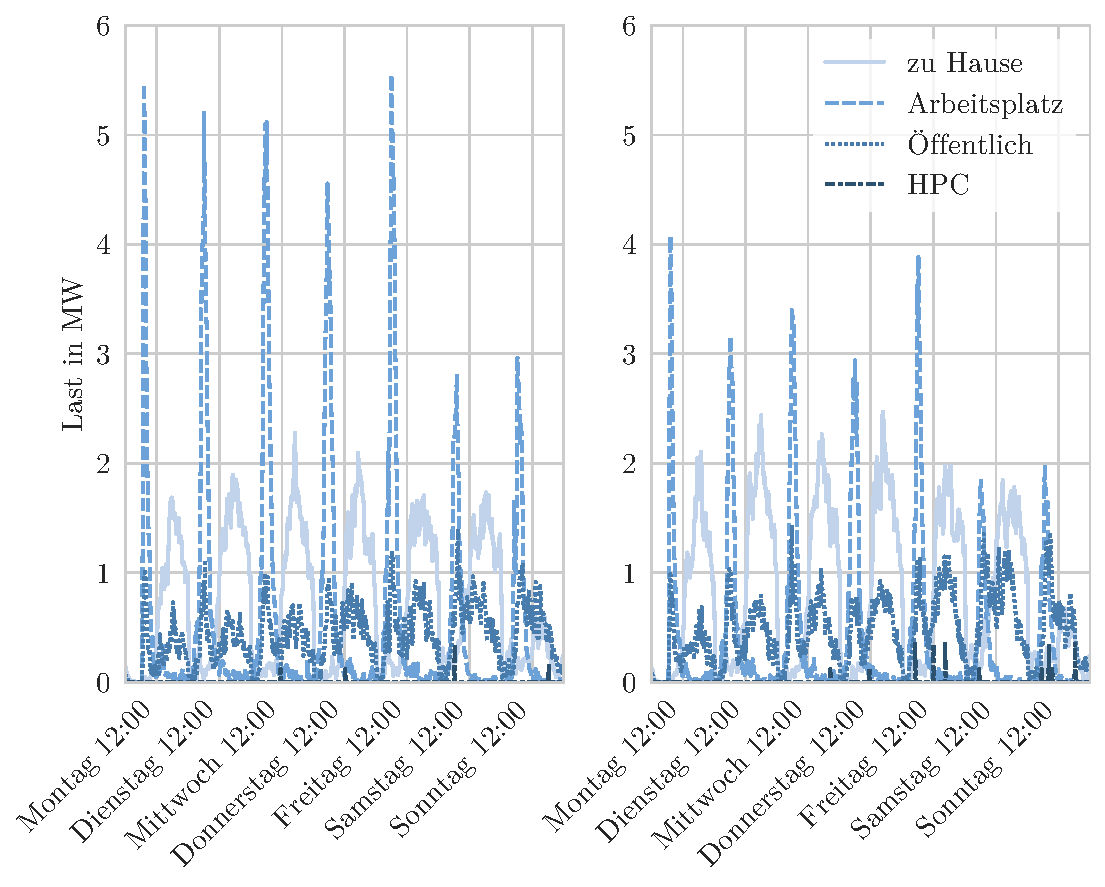
\includegraphics[width=\textwidth]{Bilder/example_load_profile}
    \caption[E-Pkw-Lastprofil für Referenz-Laden im Netz \num{176} über eine Woche im Antriebswende-Szenario und der \SzeFirmenparkplatz]{E-Pkw-Lastprofil (netzseitige Last; inkl. Umwandlungsverluste) für Referenz-Laden im Netz \(176_{\text{PV}}\) über eine Woche im Antriebswende-Szenario (links) und der \SzeFirmenparkplatz (rechts)}\label{fig:example_load_profile}
\end{figure} % TODO: Leistung statt Last

Die Lastgänge \zH und \Firmeparkplatz entsprechen den Ladevorgängen im privaten Bereich.
Unter dem Lastgang \oeffen sind hingegen alle öffentlichen Ladevorgänge mit Ausnahme der Schnellladevorgänge (\gls{HPC}) zusammengefasst.
Deutlich zu erkennen ist die hohe Gleichzeitigkeit am Vormittag sowohl an Firmenparkplätzen als auch im öffentlichen Raum, welche durch das Fahren zur Arbeit ausgelöst wird.
Auch die Rückkehr zum Wohnort ist ab dem frühen Nachmittag in den Lastgängen \zH und im öffentlichen Raum deutlich zu erkennen.
Schnellladevorgänge treten unregelmäßig im Verlauf der Woche auf.
Vor allem am Sonntag kommt es zu deutlich geringeren Anteilen von Ladevorgängen zu Hause und am Firmenparkplatz, wodurch das Flexibilisierungspotential am Wochenende geringer ausfällt.
Gegenüber dem Antriebswende-Szenario sinkt die Höchstlast in der \SzeFirmenparkplatzdot, jedoch sinkt auch das Flexibilisierungspotential bei einem annähernd gleichbleibendem Energiebedarf durch die Verschiebung der Ladevorgänge in den öffentlichen Raum.\medskip
% TODO: erwähnen, dass durch die anderen Wahrscheinlichkeiten und dem Simulieren von nur einer Woche hier leichte Differenzen auftreten und auf Steckbriefe verweisen

Die entsprechenden Dauerlastkurven für die Gemeinde über eine Woche (s. \autoref{fig:example_load_curve}) zeigen nochmals deutlich die dominante Rolle der Hochlastphase die Aufgrund der hohen Gleichzeitigkeit des Wegezwecks \Arbeit vor allem am Firmenparkplatz aber auch im öffentlichen Raum auftritt.
So wird im Antriebswende-Szenario eine Spitzenlast von \SI{14.8}{\mw} erreicht.
Im Netzgebiet \num{176} befinden sich im Antriebswende-Szenario \SI{26359}{\FZ}, welches einem Verhältnis von Spitzenlast zu Fahrzeugen von \SI{0.56}{\kWperFZ} entspricht.
Zum Vergleich wurde in der \textit{Kurzstudie Elektromobilität} für den \gls{NEP} \cite{Ebner2019} für \SI{12}{\MioStk} innerhalb eines Jahres eine Spitzenlast von \SI{12}{\gw} ermittelt, welches einem Verhältnis von \SI{1.00}{\kWperFZ} entspricht.
Für eine mittlere Woche liegt die Spitzenlast in der \textit{Kurzstudie Elektromobilität} bei \SI{9}{\gw} und somit bei \SI{0.75}{\kWperFZ}.
Die Spitzenlast wird nach der \textit{Kurzstudie Elektromobilität} in der Regel am Nachmittag erreicht, da im Vergleich zu dieser Arbeit deutlich weniger Ladevorgänge an Firmenparkplätzen stattfinden.
Hierdurch ergibt sich innerhalb der Woche am Abend eine besonders hohe Gleichzeitigkeit beim Laden \zHdot, während in der durchgeführten Simulation dieser Arbeit täglich zwei Leistungsspitzen mit einer geringeren Gleichzeitigkeit am Morgen und am Nachmittag auftreten.
Das Ergebnis liegt somit in einer ähnlichen Dimension und die Ergebnisse der Simulation können als plausibel angesehen werden.

% TODO: CP E-Bedarf je grid id und Szenario



\begin{figure}[H]
    \centering
    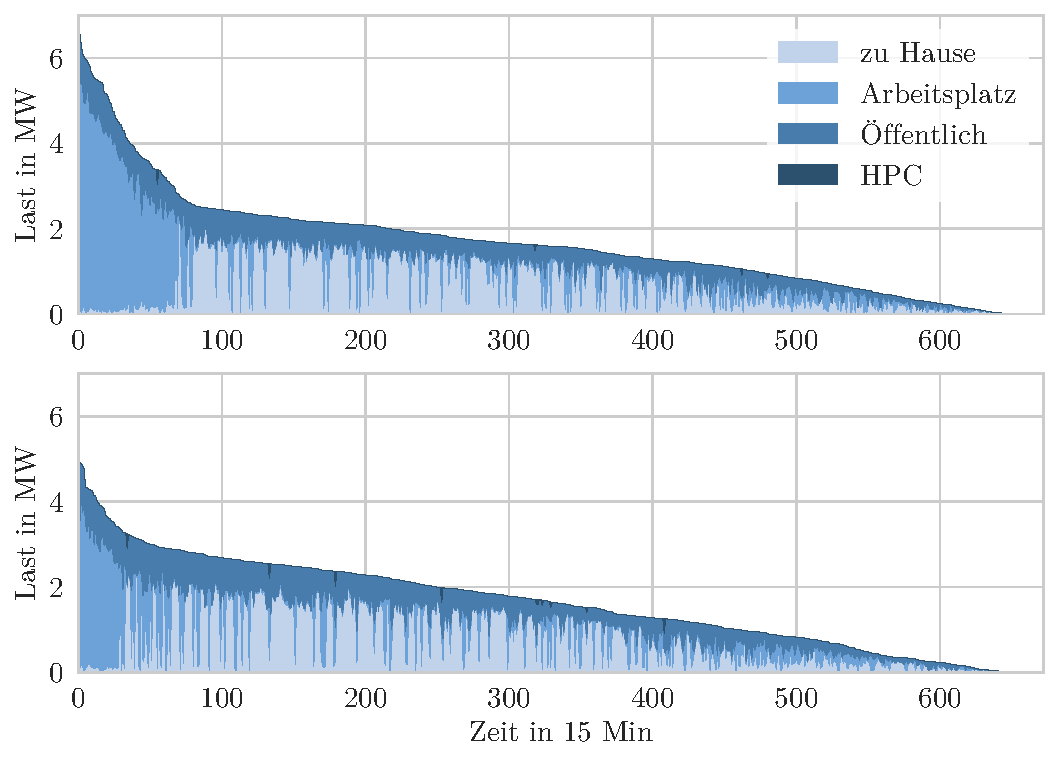
\includegraphics[width=0.9\textwidth]{Bilder/example_load_duration_curve}
    \caption{E-Pkw-Dauerlastkurve für Referenz-Laden im Netz \num{176} über eine Woche im Antriebswende-Szenario (oben) und der \SzeFirmenparkplatz (unten)}\label{fig:example_load_curve}
\end{figure} % TODO: Leistung statt Last

Zum Zeitpunkt der Erstellung der Fahrtprofile war es noch nicht möglich, einen längeren Zeitraum als eine Woche am Stück zu simulieren.
Durch die Zuordnung eines zufälligen Eingangs-\gls{SOC} für einige Fahrzeuge (s. \autoref{chap:simbev_theo}) fällt der Ladebedarf am Montag nicht deutlich aus der Reihe.
Jedoch kann hierdurch ein weiterer Effekt nitch verhindert werden.
Bei Fahrzeugen, welche weder einen festen Ladepunkt zu Hause oder an Firmenparplätzen zugewiesen bekommen haben, fällt der \gls{SOC} im Laufe der Woche langsam ab.
Hierdurch kommt es durch die Abhängigkeit der Ladewahrscheinlichkeit vom \gls{SOC} zu einer Zunahme des Ladebedarfs im öffentlichen Raum über die Woche.
Es ist zu vermuten, dass dies weiterhin dazu führt, dass Ladevorgänge an Schnellladeinfrastruktur un­ter­re­prä­sen­tiert dargestellt werden.


\subsection{Verteilung der Ladevorgänge auf die Ladeinfrastruktur}\label{chap:distribute_demand_ev}

Die Verteilung der Ladevorgänge auf eine konkrete georeferenzierte Ladeinfrastruktur nach \autoref{chap:theo_distribution} liefert je Netzgebiet eine Vielzahl von unterschiedlichen Netzanschlusspunkten.
In \autoref{fig:cps_in_grid} finden sich beispielhaft die ermittelten Netzanschlusspunkte für Ladeinfrastruktur innerhalb des Netzgebietes \num{176} für das Antriebswende-Szenario für Ladeinfrastruktur zu Hause, an Firmenparkplätzen, Normalladeinfrastruktur im öffentlichen Raum und für Schnellladeinfrastruktur (\gls{HPC}).
Es wird deutlich, dass die Ladeinfrastruktur \zH die meisten Netzanschlusspunkte aufweist, während für die Schnellladeinfrastruktur nur wenige Netzanschlusspunkte benötigt werden.

\begin{figure}[H]
    \centering
    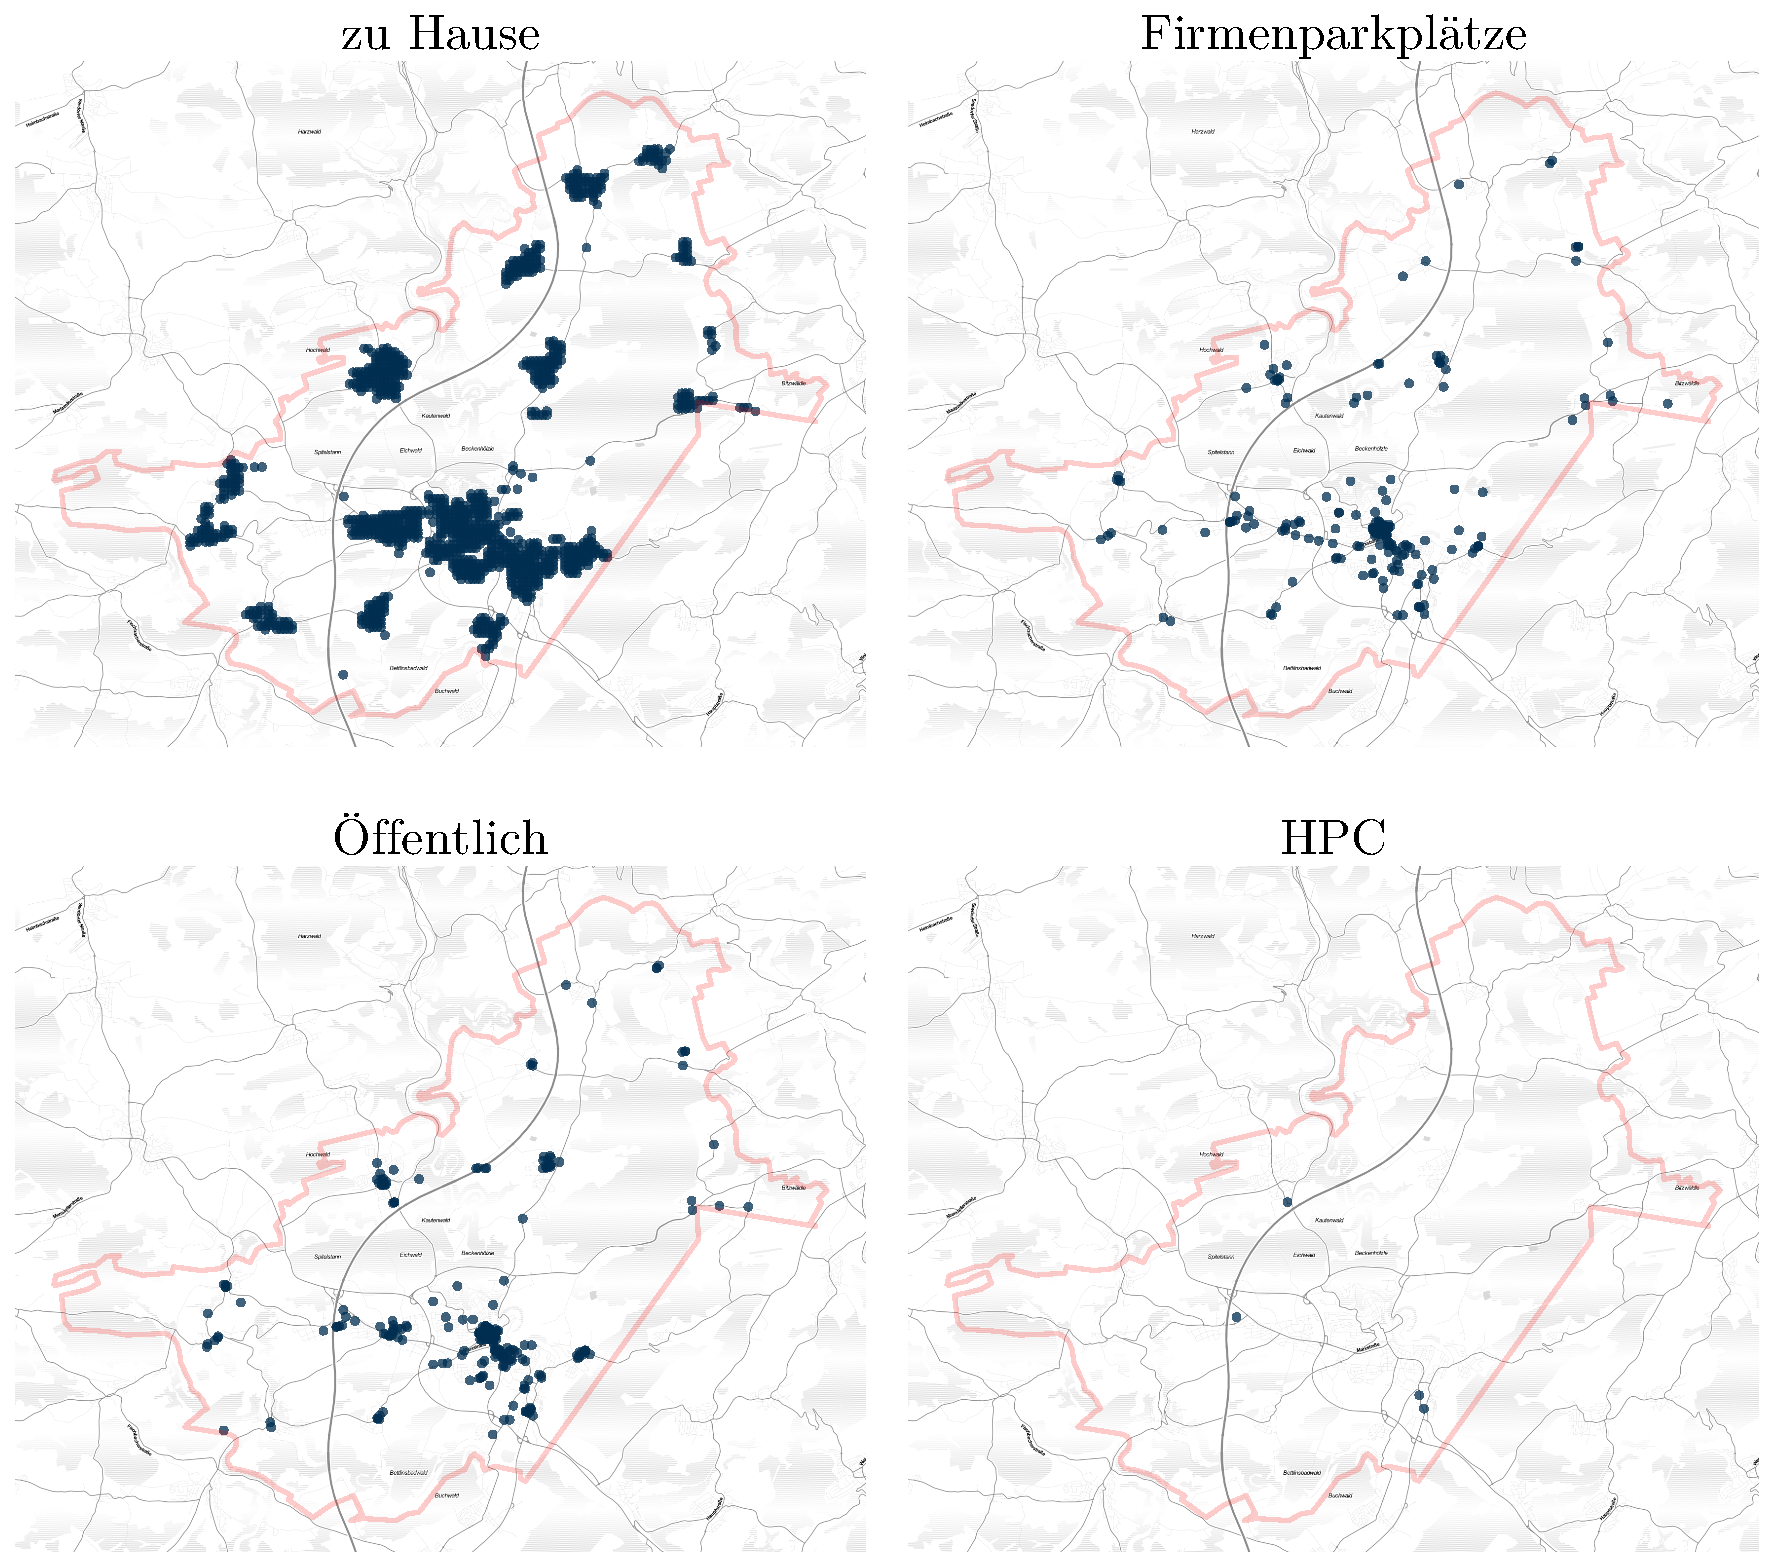
\includegraphics[width=\textwidth]{Bilder/cps_in_grid_176}
    \caption[Geographische Verteilung der ermittelten und zugewiesenen Netzanschlusspunkte für Ladeinfrastruktur im Netz \num{176} für das Antriebswende-Szenario je Lade use case]{Geographische Verteilung der ermittelten und zugewiesenen Netzanschlusspunkte für Ladeinfrastruktur im Netz \(176_{\text{PV}}\) für das Antriebswende-Szenario je Lade use case}\label{fig:cps_in_grid}
\end{figure}

Neben der geographischen Lokalisation der Ladeinfrastruktur ist es für die Netzuntersuchungen entscheidend, ob die Ladeinfrastruktur in der \gls{NS}- oder \gls{MS}-Ebene angeschlossen ist.
Wenn der Anschluss in der \gls{NS}-Ebene erfolgt, dann werden sowohl die Betriebsmittel der \gls{MS}- und \gls{MS}-Ebene belastet, während bei einem Anschluss in der \gls{MS}-Ebene auch nur diese betroffen ist.
Außerdem findet ab einem Anschluss von privater Ladeinfrastruktur in der \gls{MS}-Ebene auch bei der Referenz-Ladestrategie reduziertes Laden statt (s. \autoref{chap:theo_strategies}).
In \autoref{tab:lvConnectionShare} findet sich der Anteil des in der \gls{NS}-Ebene anfallenden Energiebedarfs vom Gesamtenergiebedarf der Ladeinfrastruktur im Netzgebiet.
Es wird deutlich, dass der Anteil von Ladeinfrastruktur in der \gls{MS}-Ebene mit einer steigenden Zahl von Fahrzeugen zunimmt.
Gleichzeitig zeigt sich, dass in der \SzeFirmenparkplatz der Anteil von Ladeinfrastruktur in der \gls{MS}-Ebene deutlich geringer ausfällt als im Antriebswende-Szenario, trotz einer gleichen Anzahl an \gls{EPKW} innerhalb der Szenarien.
Dies lässt sich damit erklären, dass neben der öffentlichen Ladeinfrastruktur vor allem Ladeinfrastruktur auf Firmenparkplätzen einen Anschluss in der \gls{MS}-Ebene benötigt.
Da im Antriebswende-Szenario mehr Ladepunkte auf eine gleichbleibende Anzahl von möglichen Anschlusspunkten für Ladeinfrastruktur auf Firmenparkplätzen verteilt werden müssen, fällt die Anschlussleistung dieser Ladeinfrastruktur deutlich höher aus und macht somit einen Anschluss in der \gls{MS}-Ebene nötig.

{
\renewcommand{\arraystretch}{1.2}% grßerer Zeilenabstand
\sisetup{range-phrase=~{--}~}% Gedankenstrich statt "bis" bei SIrange
\begin{table}[H]
	\begin{center}
		\caption{Anteil des in der NS-Ebene anfallenden Energiebedarfs vom Gesamtenergiebedarf der Ladeinfrastruktur je Szenario}
		\begin{tabu} to \textwidth {X[0.5] X[1, r] X[1, r] X[1.2, r] X[1.2, r]}
			\hline
			Netz ID    & NEP C \num{2035}    & Referenz            & Antriebswende       & \glqq Firmenparkplatz\grqq \\ \hline
			\num{176}  & \SI{98.0}{\percent} & \SI{92.9}{\percent} & \SI{82.0}{\percent} & \SI{91.3}{\percent}        \\
			\num{1056} & \SI{99.8}{\percent} & \SI{99.5}{\percent} & \SI{94.0}{\percent} & \SI{97.9}{\percent}        \\
			\num{1690} & \SI{99.8}{\percent} & \SI{97.0}{\percent} & \SI{86.5}{\percent} & \SI{92.9}{\percent}        \\
			\num{1811} & \SI{99.9}{\percent} & \SI{98.7}{\percent} & \SI{90.0}{\percent} & \SI{95.2}{\percent}        \\
			\num{177}  & \SI{96.6}{\percent} & \SI{86.8}{\percent} & \SI{77.8}{\percent} & \SI{86.7}{\percent}        \\
			\num{2534} & \SI{99.7}{\percent} & \SI{97.4}{\percent} & \SI{80.8}{\percent} & \SI{91.4}{\percent}        \\ \hline
		\end{tabu}
		\label{tab:lvConnectionShare}
	\end{center}
	\vspace{-3mm}%Put here to reduce too much white space after your table
\end{table}
}


In \autoref{tab:largestLVGridShare} ist die Anzahl an \gls{NS}-Netzen je \gls{MS}-Netzgebiet und der maximal anfallender Energieanteil eines \gls{NS}-Netzes am Gesamtenergiebedarf der Ladeinfrastruktur in der \gls{NS}-Ebene in allen betrachteten Szenarien dargestellt.
Hierbei wird deutlich, dass es in einigen \gls{MS}-Netzgebieten zu einer starken lokalen Konzentration an Ladeinfrastruktur kommt.
So entfallen beispielsweise im \gls{MS}-Netzgebiet \num{2534} im NEP C~\num{2035} Szenario \SI{62.3}{\percent} des Energiebedarfs der Ladeinfrastruktur in der \gls{NS}-Ebene innerhalb eines einzigen \gls{NS}-Netzes an.
Auch im \gls{MS}-Netzgebiet \num{176} zeigt sich eine starke lokale Konzentration innerhalb eines \gls{NS}-Netzes, welches sich in \autoref{fig:cps_in_grid} durch eine starke Konzentration der Ladeinfrastruktur in den bewohnten Regionen widerspiegelt.
In der Realität würde es bei solch starken lokalen Konzentrationen vermutlich zu einem Netzneubau kommen, welcher innerhalb dieser Arbeit nicht abgebildet werden kann.

{
\renewcommand{\arraystretch}{1.2}% grßerer Zeilenabstand
\sisetup{range-phrase=~{--}~}% Gedankenstrich statt "bis" bei SIrange
\begin{table}[H]
	\begin{center}
		\caption{Anzahl der NS-Netze je MS-Netzgebiet und maximal anfallender Energieanteil eines NS-Netzes am Gesamtenergiebedarf der Ladeinfrastruktur in den NS-Netzen in allen betrachteten Szenarien}
		\begin{tabu} to 0.7\textwidth {X[0.75] X[1, r] X[1.5, r]}
			\hline
			Netz ID    & Anzahl NS-Netze & Maximaler Energieanteil 			\\ \hline
			\num{176}  & \num{105}       & \SI{36.3}{\percent}              \\
			\num{1056} & \num{130}       & \SI{12.9}{\percent}              \\
			\num{1690} & \num{179}       & \SI{11.4}{\percent}              \\
			\num{1811} & \num{381}       & \SI{7.9}{\percent}               \\
			\num{177}  & \num{56}        & \SI{26.5}{\percent}              \\
			\num{2534} & \num{9}         & \SI{62.3}{\percent}              \\ \hline
		\end{tabu}
		\label{tab:largestLVGridShare}
	\end{center}
	\vspace{-3mm}%Put here to reduce too much white space after your table
\end{table}
}


\subsection{Ergebnisse der Implementierung der Ladestrategien}\label{chap:results_charging_strategies}

Im Rahmen der Netzuntersuchungen kommt den Zeitreihen der Last der \glspl{EPKW} die größte Bedeutung zu, da die Last und Erzeugung aller anderen Verbraucher und Erzeuger nicht veränderlich ist.
Das Ziel der Ladestrategien (s. \autoref{chap:theo_strategies}) ist es, die Netzbelastung möglichst gering zu halten.
Bei den Ladegruppen und reduzierten Laden soll dies durch ein präventives Lademanagement und bei dem Residuallast-Laden durch ein aktives Lademanagement erreicht werden.

\begin{figure}[H]
    \centering
    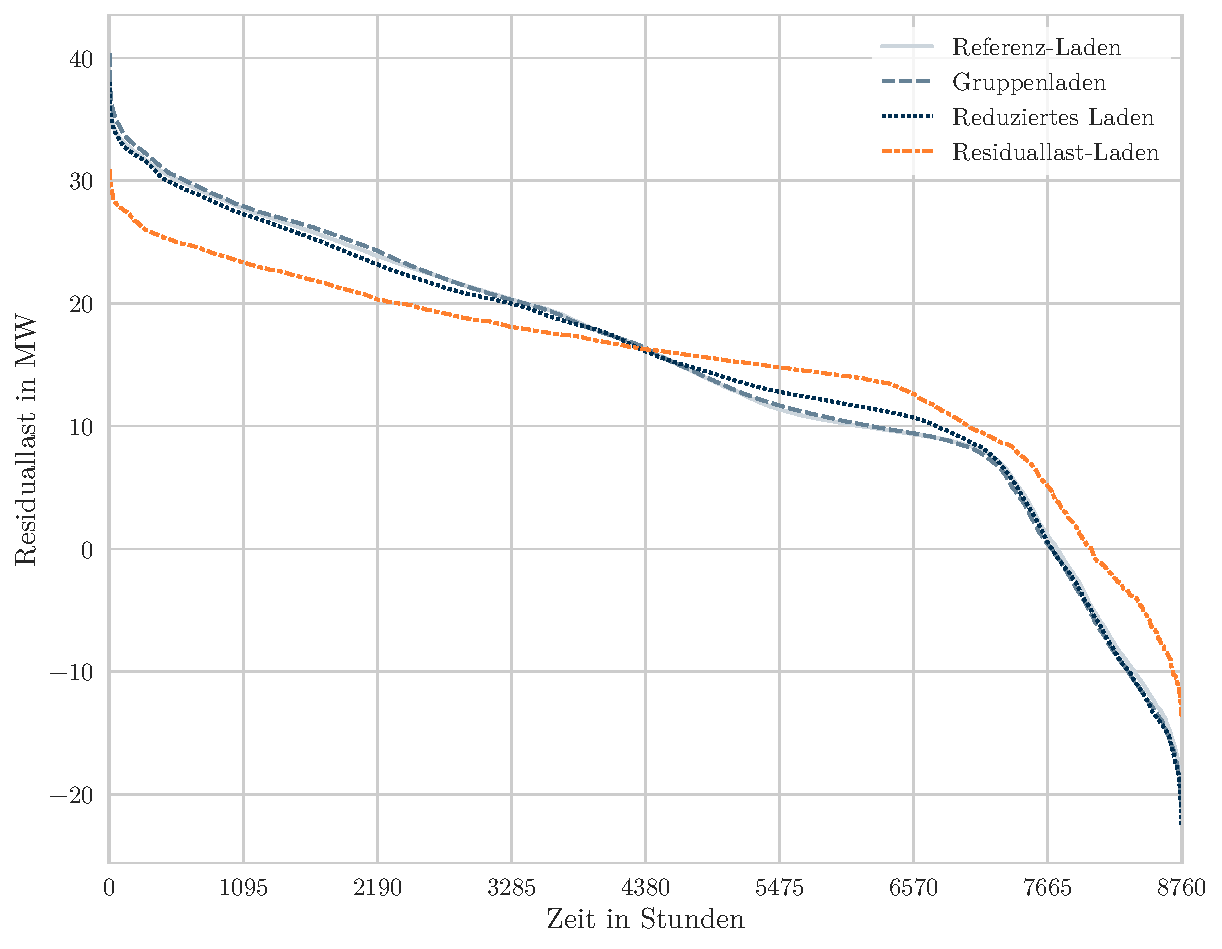
\includegraphics[width=1\textwidth]{Bilder/example_resiual_load}
    \caption{Residuallast im Netzgebiet \num{176} für das Antriebswende-Szenario}\label{fig:residual_load}
\end{figure}

\autoref{fig:residual_load} zeigt beispielhaft für das Netzgebiet \num{176} die Abhängigkeit der Residuallast von der Ladestrategie im Antriebswende-Szenario.
Dabei zeigt sich, dass vor allem die Residuallast-Ladestrategie zu einer klaren Glättung der Residuallastkurve führt, während sich bei den sonstigen Ladestrategien ein ähnliches Bild zeigt.
Dabei führen die Ladegruppen gegenüber dem Referenz-Laden sogar zu einem gegensätzlichen Effekt und zu einer Erhöhung der Spitzenlast im Last- und Rückspeisefall.
In \autoref{fig:residual_load_diff} ist die Veränderung der Residuallast über ein Jahr in Abhängigkeit von den verschiedenen Ladestrategien dargestellt.
Dabei zeigt die Darstellung der Referenz-Ladestrategie (oben links) die Residuallast über ein Jahr, während in den anderen drei Darstellungen die Differenz der jeweiligen Ladestrategie zum Referenz-Laden abgebildet wird.
Bei den Ladegruppen zeigt sich gegenüber dem Referenz-Laden eine deutlich stärkere Belastung am Vormittag und ein Abfallen der Belastung bis zum Mittag.
Am Nachmittag lässt sich in der Regel keine Differenz feststellen.
Bei der reduzierten Ladestrategie kommt es zu einer leicht reduzierten Residuallast im Verlauf des Tages, während die Residuallast Nachts leicht zunimmt.
Die stärksten Veränderungen werden bei der Residuallast-Ladestrategie festgestellt.
Da es sich bei dem Netzgebiet \num{176} um ein \gls{PV}-dominiertes Netz handelt, kommt es zu einer starken Verschiebung der Ladevorgänge in die Mittagszeit.
Auch kommt es zu einer deutlichen Verschiebung der Last in die Schwachlastzeit nach Mitternacht, während die Residuallast am Vor- und Nachmittag abnimmt.
Da auf diese weise jedoch nur Aussagen über das komplette \gls{MS}-Netzgebiet getroffen werden können, kann hier draus noch keine Aussage über die Belastung der einzelnen Betriebsmittel getroffen werden.

\begin{figure}[H]
    \centering
    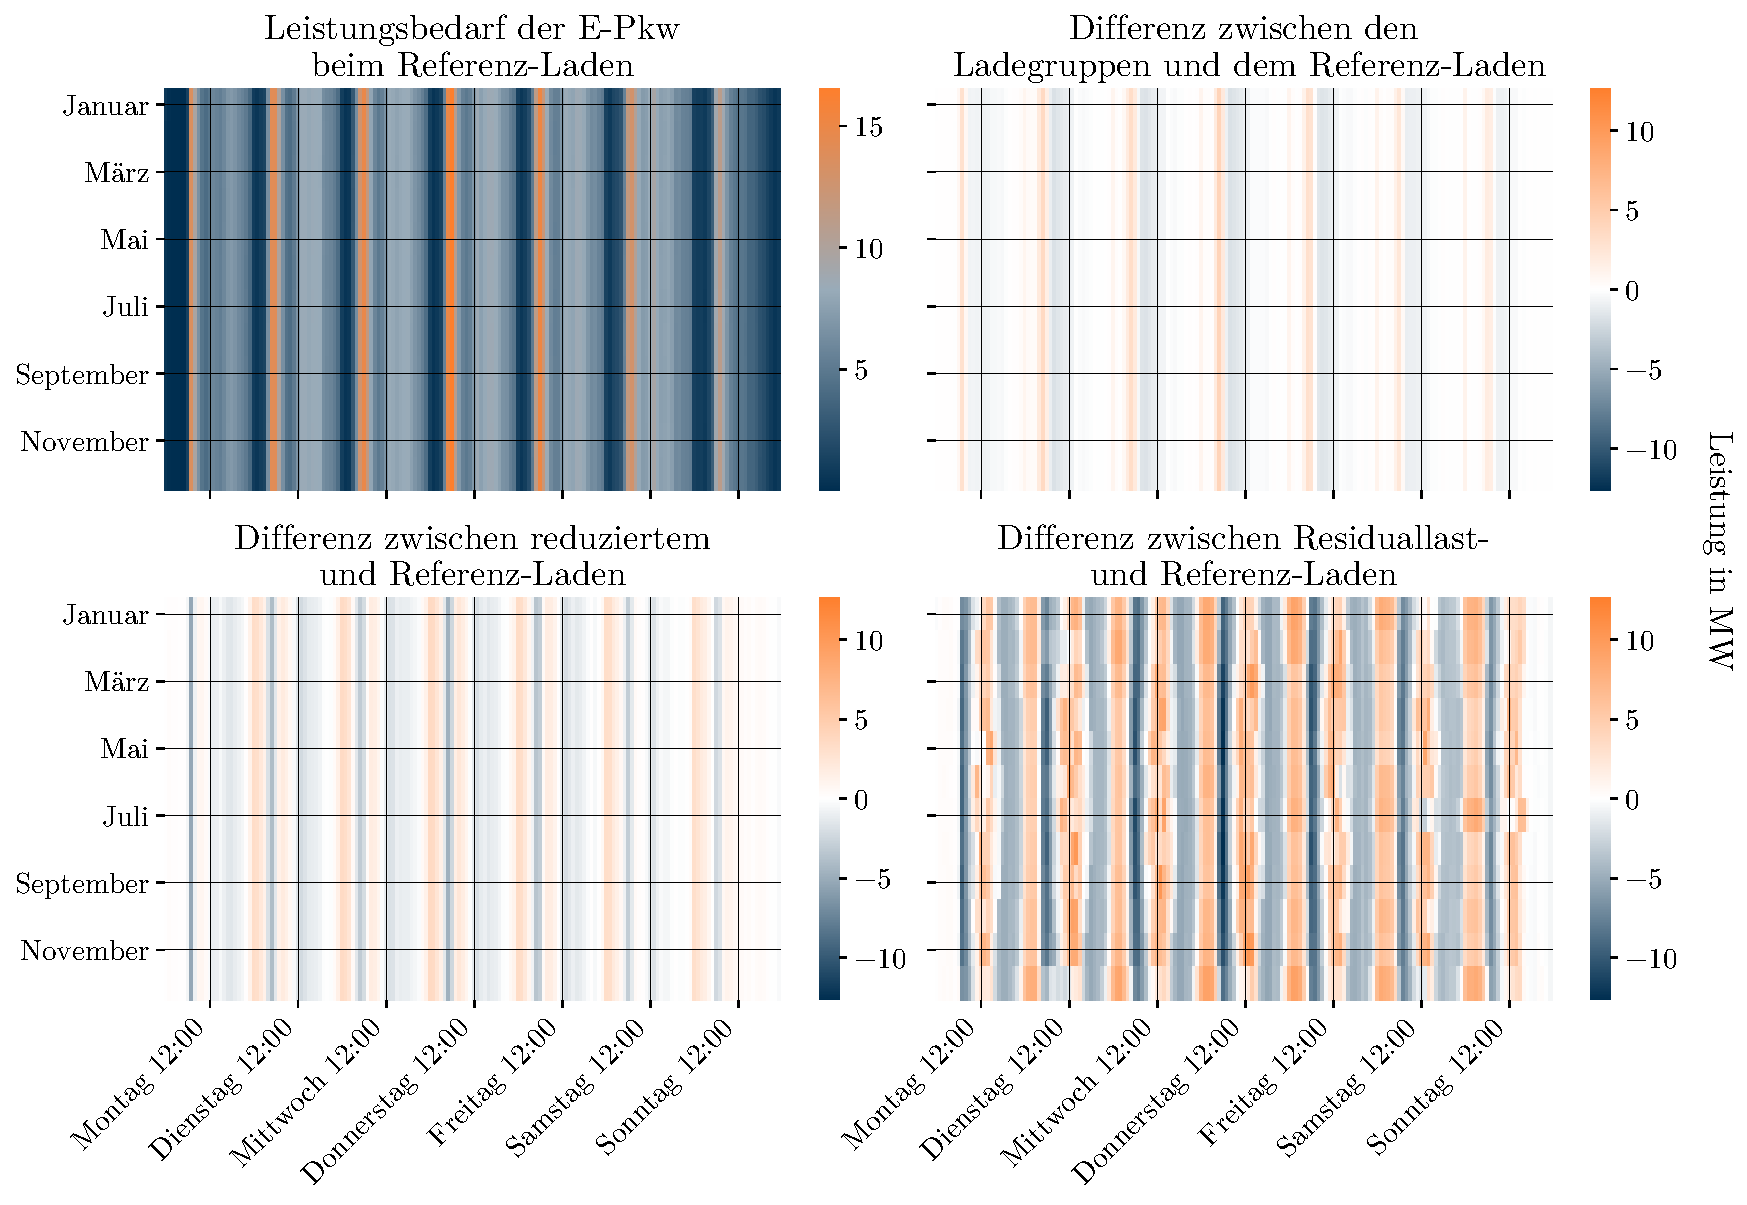
\includegraphics[width=\textwidth]{Bilder/residual_load_diff}
    \caption[Veränderung des durchschnittlichen stündlichen Leistungsbedarfs von E-Pkw je Wochentag im Netz \num{176} für das Antriebswende-Szenario über ein Jahr in Abhängigkeit von der Ladestrategie]{Veränderung des durchschnittlichen stündlichen Leistungsbedarfs von E-Pkw je Wochentag im Netz \(176_{\text{PV}}\) für das Antriebswende-Szenario über ein Jahr in Abhängigkeit von der Ladestrategie}\label{fig:residual_load_diff}
\end{figure}

% TODO: Eventuell Auswertung, wie sich die Residuallast durch das Residuallast-Laden verändert bei den unterschiedlichen Netzgebieten und Szenarien
% TODO: Bubble maps


\subsection{Abregelungsbedarf innerhalb der untersuchten Netzgebiete}

In diesem Abschnitt werden die Ergebnisse der Ermittlung des Abregelungsbedarfs innerhalb der sechs untersuchten Netzgebiete dargestellt.
Dabei wird getrennt auf die drei Netz-Kategorien \gls{PV}-, Wind- und Last-dominiert eingegangen, um eine Aussage über die Wirksamkeit der Ladestrategien innerhalb der verschiedenen Netz-Kategorien treffen zu können.
Hierzu werden die zwei Wochen mit der minimalen (kurz: Woche~A) bzw. maximalen (kurz: Woche~B) durchschnittliche Residuallast je Netz untersucht, um eine möglichst hohe Bandbreite an Einspeise- und Lastfällen abzudecken.
Die entsprechenden Zeiträume finden sich in \autoref{tab:extreme_weeks}, wobei die untersuchten Wochen und das fiktive betrachtete Jahr mit einem Montag beginnen.

{
\renewcommand{\arraystretch}{1.2}% grßerer Zeilenabstand
\sisetup{range-phrase=~{--}~}% Gedankenstrich statt "bis" bei SIrange
\begin{table}[H]
	\begin{center}
		\caption{Untersuchte Wochen je Netzgebiet}
		\begin{tabu} to 0.6\textwidth {X[0.5] X[1, r] X[1, r]}
			\toprule
			Netz ID	   & Woche A                         & Woche B                         \\ \midrule
			\num{176}  & \(16.04. \text{ {--} } 22.04.\) & \(08.01. \text{ {--} } 14.01.\) \\
			\num{1056} & \(30.04. \text{ {--} } 06.05.\) & \(08.01. \text{ {--} } 14.01.\) \\
			\num{1690} & \(03.12. \text{ {--} } 09.12.\) & \(29.10. \text{ {--} } 04.11.\) \\
			\num{1811} & \(10.12. \text{ {--} } 16.12.\) & \(24.09. \text{ {--} } 30.09.\) \\
			\num{177}  & \(16.04. \text{ {--} } 22.04.\) & \(10.12. \text{ {--} } 16.12.\) \\
			\num{2534} & \(16.04. \text{ {--} } 22.04.\) & \(03.12. \text{ {--} } 09.12.\) \\ \bottomrule
		\end{tabu}
		\label{tab:extreme_weeks}
	\end{center}
	\vspace{-3mm}%Put here to reduce too much white space after your table
\end{table}
}

Innerhalb der betrachteten Szenarien, Ladestrategien und Wochen schwankt der Abregelungsbedarf von nicht-\glspl{FEE} Anlagen nur in einem sehr geringen Maße, weshalb der Fokus erzeugungsseitig auf den \gls{FEE} Anlagen liegt.
Dies lässt sich dadurch begründen, dass die Abregelung der nicht-\gls{FEE} Anlagen in den betrachteten Netzgebieten in der Regel aufgrund von Restriktionen in der \gls{NS}-Ebene erfolgt.
Da es sich bei den nicht-\gls{FEE} Anlagen ausschließlich um Biomasse- und Wasserkraftwerke handelt, findet sich innerhalb der betroffenen \gls{NS}-Netze in der Regel keine oder nur wenig Ladeinfrastruktur für \gls{EPKW}.
Hierdurch kommt es nur sehr selten zu einem Einfluss auf den Abregelungsbedarf von nicht-\gls{FEE} Anlagen.
Die vollständigen Ergebnisse für die Ermittlung des Abregelungsbedarfs finden sich im Anhang in den Netz-Steckbriefen ab {\color{red} TODO}.


\subsubsection{PV-dominierte Netze}

Die \gls{PV}-dominierten Netze \num{176} und \num{1056} besitzen stark unterschiedliche Charakteristika.
So weist das Netz \num{176} im Antriebswende-Szenario in der Woche~A (minimale Residuallast) ein Verhältnis zwischen der Einspeisung von \glspl{FEE} und dem Ladebedarf der \glspl{EPKW} von etwa \(2:1\) auf, während dieses Verhältnis im Netz \num{1056} bei etwa \(11:1\) liegt.
Auch weist das Netz \num{176} eine deutlich größere Einspeisung von nicht-\gls{FEE} Anlagen auf und der Verbrauch der sonstigen Lasten ist mehr als dreimal so hoch als im Netz \num{1056}.
Eine Auflistung der wichtigsten Eckdaten für die Woche~A beider Netze findet sich in \autoref{tab:pv_dominated_week_a_char} und der Ladebedarf im Netzgebiet je Szenario findet sich in \autoref{tab:pv_dominated_epkw_demand}.

{
\renewcommand{\arraystretch}{1.2}% grßerer Zeilenabstand
\sisetup{range-phrase=~{--}~}% Gedankenstrich statt "bis" bei SIrange
\begin{table}[H]
	\begin{center}
		\caption{Einspeisung von fEE und nicht-fEE Anlagen sowie der Bedarf von sonstigen Lasten in den PV-dominierten Netzen}
		\begin{tabu} to 0.7\textwidth {X[2] X[1, r] X[1, r]}
			\toprule
											  & Netz \num{176} & Netz \num{1056} \\ \midrule
			Einspeisung fEE in \si{\mwh}      & \num{2262.2}   & \num{4054.8}    \\
			Einspeisung Sonstige in \si{\mwh} & \num{1459.8}   & \num{254.5}     \\
			Bedarf Sonstige  in \si{\mwh}     & \num{4196.8}   & \num{1318.0}    \\ \bottomrule
		\end{tabu}
		\label{tab:pv_dominated_week_a_char}
	\end{center}
	\vspace{-3mm}%Put here to reduce too much white space after your table
\end{table}
}

{
\renewcommand{\arraystretch}{1.2}% grßerer Zeilenabstand
\sisetup{range-phrase=~{--}~}% Gedankenstrich statt "bis" bei SIrange
\begin{table}[H]
	\begin{center}
		\caption{Ladebedarf der E-Pkw in den PV-dominierten Netzen je Szenario}
		\begin{tabu} to 0.6\textwidth {X[1.5] X[1, r] X[1, r]}
			\toprule
			Ladebedarf in   \si{\mwh} 		& Netz \num{176} & Netz \num{1056} \\ \midrule
			NEP C~\num{2035}                & \num{290.0}    & \num{109.3}     \\
			Referenz                        & \num{519.6}    & \num{193.7}     \\
			Antriebswende                   & \num{987.7}    & \num{368.5}     \\
			\glqq Firmenparkplatz\grqq{}    & \num{974.3}    & \num{363.1}     \\ \bottomrule
		\end{tabu}
		\label{tab:pv_dominated_epkw_demand}
	\end{center}
	\vspace{-3mm}%Put here to reduce too much white space after your table
\end{table}
}

In \autoref{tab:pv_dominated_week_a_epkw_cur} findet sich der ermittelte Abregelungsbedarf des Ladebedarfs und in \autoref{tab:pv_dominated_week_a_load_cur} der sonstigen Lasten für die Netze \num{176} und \num{1056} für die Referenz-Ladestrategie.
Der Abregelungsbedarf von Lasten nimmt erwartungsgemäß mit dem Hochlauf an \gls{EPKW} zu.
Im Netz \num{176} kommt es zu einer extrem hohen Abregelung von bis zu knapp \SI{50}{\percent} des gesamten Ladebedarfs der \gls{EPKW}.
Dieser Abregelungsbedarf entsteht beispielsweise in der \SzeFirmenparkplatz zu etwa \SI{82}{\percent} innerhalb von nur drei \gls{NS}-Netzen, welches somit die extreme Konzentration des Ladebedarfs innerhalb des Netzes \num{176} nach \autoref{tab:largestLVGridShare} widerspiegelt.
Dieser Effekt lässt sich auch auf die anderen Szenarien übertragen.\medskip

Demgegenüber erweist sich das Netz \num{1056} als deutlich stabiler und weist nur einen geringen Abregelungsbedarf des Ladebedarfs von \gls{EPKW} auf.
Aufgrund der geringeren Anzahl an Lademöglichkeiten auf Firmenparkplätzen in der \SzeFirmenparkplatzdot, werden die Ladevorgänge gleichmäßiger über den Tag verteilt (vgl. \autoref{fig:example_load_profile} und \autoref{fig:example_load_curve}).
Zusätzlich fällt der Ladebedarf aufgrund der probabilistischen Natur der Simulation und der veränderten Eingangsparameter in der \SzeFirmenparkplatz geringer aus als im Antriebswende-Szenario.
Aus diesen Gründen fällt der Abregelungsbedarf im Netz \num{1056} geringer aus als im Antriebswende-Szenario.
Da im Netz \num{176} vor allem \gls{NS}-Netze mit einem hohen Anteil an Ladevorgängen zu Hause von den starken Abregelungen betroffen sind, tritt in diesem Netz ein gegenteiliger Effekt auf und der Abregelungsbedarf erhöht sich in der \SzeFirmenparkplatzdot.

{
\renewcommand{\arraystretch}{1.2}% grßerer Zeilenabstand
\sisetup{range-phrase=~{--}~}% Gedankenstrich statt "bis" bei SIrange
\begin{table}[H]
	\begin{center}
		\caption{Abregelungsbedarf des Ladebedarfs von E-Pkw in den PV-dominierten Netzen je Szenario für die Referenz-Ladestrategie in Woche A}
		\begin{tabu} to 0.6\textwidth {X[1.5] X[1, r] X[1, r]}
			\toprule
			Abregelung in   \si{\mwh}    & Netz \num{176} & Netz \num{1056} \\ \midrule
			NEP C~\num{2035}             & \num{91.2}     & \num{3.3}       \\
			Referenz                     & \num{212.7}    & \num{12.0}      \\
			Antriebswende                & \num{418.1}    & \num{31.9}      \\
			\glqq Firmenparkplatz\grqq{} & \num{470.8}    & \num{24.5}      \\ \bottomrule
		\end{tabu}
		\label{tab:pv_dominated_week_a_epkw_cur}
	\end{center}
	\vspace{-3mm}%Put here to reduce too much white space after your table
\end{table}
}

{
\renewcommand{\arraystretch}{1.2}% grßerer Zeilenabstand
\sisetup{range-phrase=~{--}~}% Gedankenstrich statt "bis" bei SIrange
\begin{table}[H]
	\begin{center}
		\caption{Abregelungsbedarf der sonstigen Lasten in den PV-dominierten Netzen je Szenario für die Referenz-Ladestrategie in Woche A}
		\begin{tabu} to 0.6\textwidth {X[1.5] X[1, r] X[1, r]}
			\toprule
			Abregelung in \si{\mwh} & Netz \num{176} & Netz \num{1056} \\ \midrule
			NEP C~\num{2035}                          &                & \num{16.2}      \\
			Referenz                                  &                & \num{19.6}      \\
			Antriebswende                             &                & \num{29.0}      \\
			\glqq Firmenparkplatz\grqq{}              &                & \num{22.9}      \\ \bottomrule
		\end{tabu}
		\label{tab:pv_dominated_week_a_load_cur}
	\end{center}
	\vspace{-3mm}%Put here to reduce too much white space after your table
\end{table}
}

In \autoref{fig:176_1056_cur_load_grid_week_A} findet sich der Einfluss der Ladestrategien auf den Abregelungsbedarf der Lasten (inkl. E-Pkw) für die Netze \num{176} und \num{1056}.
Hierbei zeigt sich, dass das Gruppenladen gegenüber der Referenz-Ladestrategie in beiden Netzen keine nennenswerten Vorteile aufweist, während durch das reduzierte Laden der Abregelunsgebdarf deutlich gesenkt werden kann.

\begin{figure}[H]
    \centering
    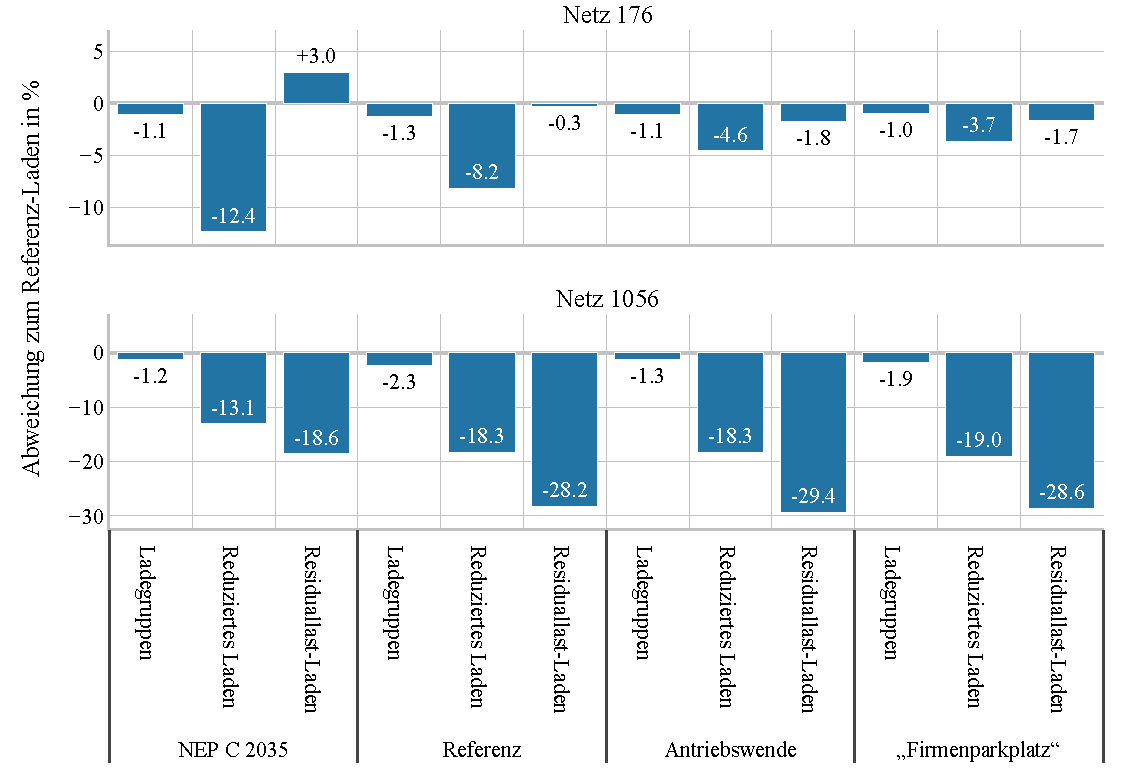
\includegraphics[width=\textwidth]{Bilder/176_1056_cur_load_grid_week_A}
    \caption[Prozentuale Veränderung des Abregelungsbedarfs von allen Lasten in Abhängigkeit von der Ladestrategie in Woche~MIN gegenüber dem Abregelungsbedarf für die Referenz-Ladestrategie je Szenario für die Netze \num{176} und \num{1056}]{Prozentuale Veränderung des Abregelungsbedarfs von allen Lasten in Abhängigkeit von der Ladestrategie in Woche~MIN gegenüber dem Abregelungsbedarf für die Referenz-Ladestrategie je Szenario für die Netze \(176_{\text{PV}}\) (oben) und \(1056_{\text{PV}}\) (unten)}\label{fig:176_1056_cur_load_grid_week_A}
\end{figure}

Im Netz \num{176} nimmt der Nutzen des reduzierten Ladens mit dem Hochlauf an \gls{EPKW} immer weiter ab, während im Netz \num{1056} der Nutzen auf einem sehr konstanten Niveau verläuft.
In \autoref{fig:176_load_curtailment_per_strategy} findet sich die durchschnittliche Abregelung von Lasten im NEP C~\num{2035} Szenario und Antriebswende-Szenario im Netz \num{176}.
Es zeigt sich, dass im NEP C~\num{2035} Szenario noch erfolgreich Last vom Nachmittag und Abend in die Nacht verschoben werden kann, ohne den Abregelungsbedarf nachts zu erhöhen.
Im Antriebswende-Szenario ist dies nicht mehr möglich und es kommt auch beim reduzierten Laden nachts zu einem stark erhöhten Abregelungsbedarf.
So wird in diesen Fällen die Abregelung nur zeitlich vom Nachmittag und Abend auf die Nacht verschoben, aber relativ kann nur ein geringer Anteil an Abregelung vermieden werden.
Demgegenüber kann im NEP C~\num{2035} noch eine größere Menge an Abregelung vor allem am Morgen verhindert werden, als am Vormittag dann vermehrt anfällt.
Dies ist im Netz \num{1056} in allen Szenarien der Fall, weshalb das reduzierte Laden immer ähnliche Erfolge mit sich bringt.\medskip

Durch das Residuallast-Laden kann der Abregelungsbedarf im Netz \num{1056} noch deutlich stärker gesenkt werden als durch das reduzierte Laden.
In dem stark \gls{PV}-dominierten Netz \num{1056} können im Antriebswende-Szenario sogar \SI{29.4}{\percent} der Abregelung durch die Residuallast-Ladestrategie verhindert werden, da die entsprechenden \gls{NS}-Netzkapazitäten für eine starke Verschiebung der Last gegeben sind und viele Erzeugerkapazitäten in der \gls{NS}-Ebene angeschlossen sind.
Im Netz \num{176} wird die Last hingegen meist in Zeiten verschoben, in denen es schon zu Abregelungen kommt, weshalb der Einfluss auf den gesamten Abregelungsbedarf sehr gering ausfällt.

\begin{figure}[H]
    \centering
    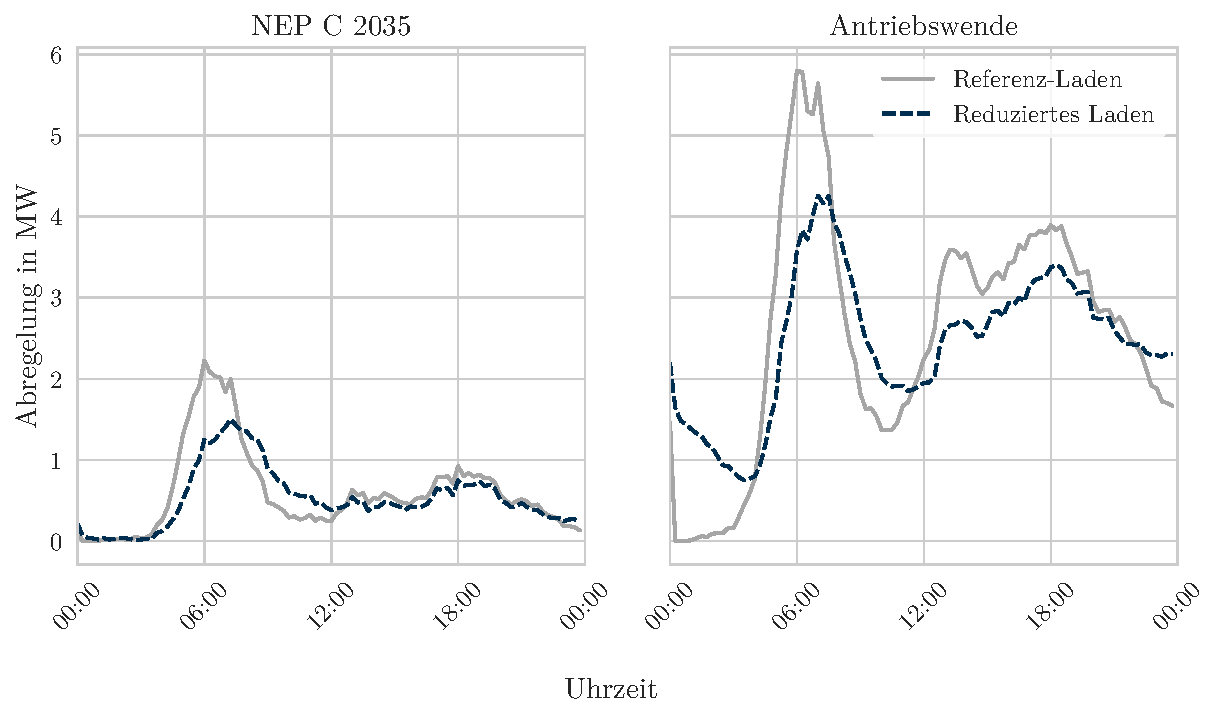
\includegraphics[width=\textwidth]{Bilder/176_load_curtailment_per_strategy}
    \caption{Durchschnittliche Abregelung von Lasten im NEP C~\num{2035} Szenario (links) und Antriebswende-Szenario (rechts) innerhalb von Woche~MIN im Netz \num{176}}\label{fig:176_load_curtailment_per_strategy}
\end{figure}

In Woche~B fällt der Abregelungsbedarf der Lasten beim Referenz-Laden im Netz \num{176} mit \SIrange{115}{503}{\mwh} und im Netz \num{1056} mit \SIrange{79}{149}{\mwh} erwartungsgemäß höher aus als in Woche~A.
Das Netz \num{176} weist nach \autoref{fig:176_1056_cur_load_grid_week_B} ein sehr ähnliches Verhalten wie in Woche~A auf.
So kann vor allem in Szenarien mit einem niedrigeren Hochlauf an \gls{EPKW} Abregelung durch das reduzierte Laden verhindert werden.
Die beiden anderen Ladestrategien zeigen in der Regel nur einen minimalen Einfluss auf den Abregelungsbedarf.
Nur im NEP C~\num{2035} Szenario erhöht sich der Abregelungsbedarf durch das Residuallast-Laden deutlich, da ein hoher Anteil des Ladebedarfs in den frühen Nachmittag verschoben wird und so eine hohe Gleichzeitigkeit entsteht.
Da im NEP C~\num{2035} Szenario noch einige Zeitschritte ohne lastseitigen Abregelungsbedarf bestehen, wird auf diese Weise auch Last aus diesen Zeitschritten in Zeitschritte mit Abregelungsbedarf verschoben, wodurch sich dieser insgesamt erhöht.\medskip

Im Netz \num{1056} kann hingegen der Abregelungsbedarf durch das Residuallast-Laden um bis zu \SI{10.5}{\percent} gesenkt werden.
Aufgrund der Zunahme der zur Verfügung stehenden flexiblen Leistung und Energie der \gls{EPKW} mit den Szenarien, kann auch immer stärker eine Glättung der Residuallast erreicht werden.
Hierdurch werden sowohl im Netz \num{1056} als auch im Netz \num{176} zunehmenden immer mehr Zeitschritte zum Laden verwendet und die temporale Konzentration von Ladevorgängen innerhalb einiger weniger Zeitschritte nimmt im Vergleich ab, wodurch sich die Effektivität des Residuallast-Ladens mit den Szenarien graduell erhöht.

\begin{figure}[H]
    \centering
    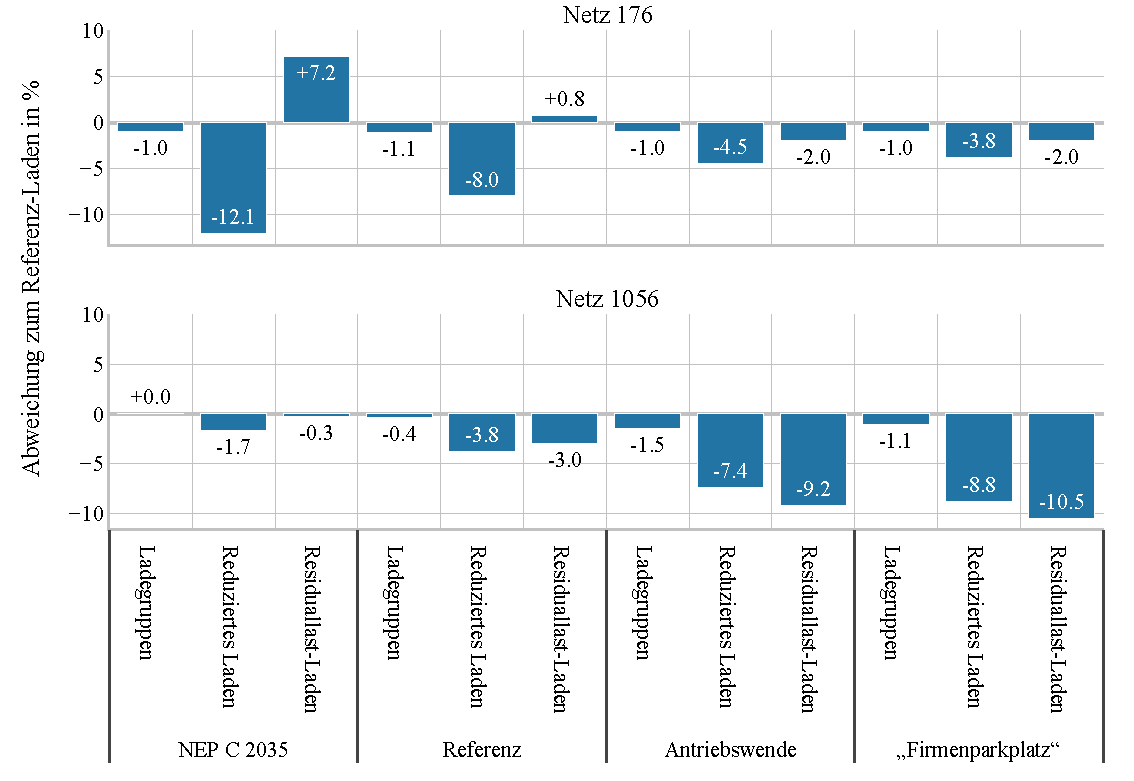
\includegraphics[width=\textwidth]{Bilder/176_1056_cur_load_grid_week_B}
    \caption[Prozentuale Veränderung des Abregelungsbedarfs von allen Lasten in Abhängigkeit von der Ladestrategie in Woche~MAX gegenüber dem Abregelungsbedarf für die Referenz-Ladestrategie je Szenario für die Netze \num{176} und \num{1056}]{Prozentuale Veränderung des Abregelungsbedarfs von allen Lasten in Abhängigkeit von der Ladestrategie in Woche~MAX gegenüber dem Abregelungsbedarf für die Referenz-Ladestrategie je Szenario für die Netze \(176_{\text{PV}}\) (oben) und \(1056_{\text{PV}}\) (unten)}\label{fig:176_1056_cur_load_grid_week_B}
\end{figure}


Bei den \gls{FEE} Anlagen zeigt sich, dass innerhalb von Woche~B in beiden \gls{PV}-dominierten Netzen keine Abregelung von \gls{FEE} Anlagen nötig ist, weshalb eine Betrachtung der Woche~B entfällt.
In Woche~A sinkt nach \autoref{tab:pv_dominated_week_a_fee_cur} der Abregelungsbedarf mit einem steigenden Hochlauf an \gls{EPKW}.
Dabei fällt auf, dass der Abregelungsbedarf von \gls{FEE} Anlagen in der \SzeFirmenparkplatz stärker abfällt als im Antriebswende-Szenario.
Dies lässt sich dadurch begründen, dass durch den höheren Anteil an Ladevorgängen im öffentlichen Raum und zu Hause nach \autoref{fig:example_load_profile} mehr Ladevorgänge in den zeitlichen Bereich hoher Einspeisung am frühen Nachmittag fallen und somit ein besserer Ausgleich zwischen Angebot und Nachfrage entsteht.

{
\renewcommand{\arraystretch}{1.2}% grßerer Zeilenabstand
\sisetup{range-phrase=~{--}~}% Gedankenstrich statt "bis" bei SIrange
\begin{table}[H]
	\begin{center}
		\caption{Abregelungsbedarf von fEE Anlagen in den Netzen \num{176} und \num{1056} je Szenario für die Referenz-Ladestrategie}
		\begin{tabu} to 0.6\textwidth {X[1.5] X[1, r] X[1, r]}
			\toprule
			Abregelung in   \si{\mwh} & Netz \num{176} & Netz \num{1056} \\ \midrule
			NEP C~\num{2035}              &                & \num{88.8}      \\
			Referenz                      &                & \num{84.3}      \\
			Antriebswende                 &                & \num{76.0}      \\
			\glqq Firmenparkplatz\grqq{}  &                & \num{73.6}      \\ \bottomrule
		\end{tabu}
		\label{tab:pv_dominated_week_a_fee_cur}
	\end{center}
	\vspace{-3mm}%Put here to reduce too much white space after your table
\end{table}
}

\autoref{fig:176_1056_cur_fee_grid_week_A} zeigt die prozentuale Veränderung des Abregelungsbedarfs von \gls{FEE} Anlagen in Abhängigkeit von der Ladestrategie.
So kann der Abregelungsbedarf durch die Residuallast-Ladestrategie im Netz \num{1056} um bis zu \SI{10.7}{\percent} und im Netz \num{176} aufgrund des geringeren Verhältnisses zwischen Einspeisung und Ladebedarf sogar um bis zu \SI{20.3}{\percent} gesenkt werden.
Demgegenüber wird durch das Gruppenladen und das reduzierte Laden der Abregelungsbedarf in der Regel erhöht.
Da im Antriebswende-Szenario deutlich mehr flexible Leistung und Energie durch \gls{EPKW} zur Verfügung steht, kann innerhalb dieses Szenarios die stärkste Reduktion erreicht werden.
Weiterhin finden gegenüber der \SzeFirmenparkplatz mehr flexible Ladevorgänge statt (vgl. \autoref{tab:ChargingShare}) vor allem auf Firmenparkplätzen statt.
Da innerhalb der Standzeiten auf Firmenparkplätzen in der Regel auch die Hochzeiten der Einspeisung von \glspl{PVA} liegen, bietet dieses Szenario in beiden Netzen ein um mehr als \SI{30}{\percent} größeres Einsparpotential beim Abregelungsbedarf von \gls{FEE} Anlagen.

\begin{figure}[H]
    \centering
    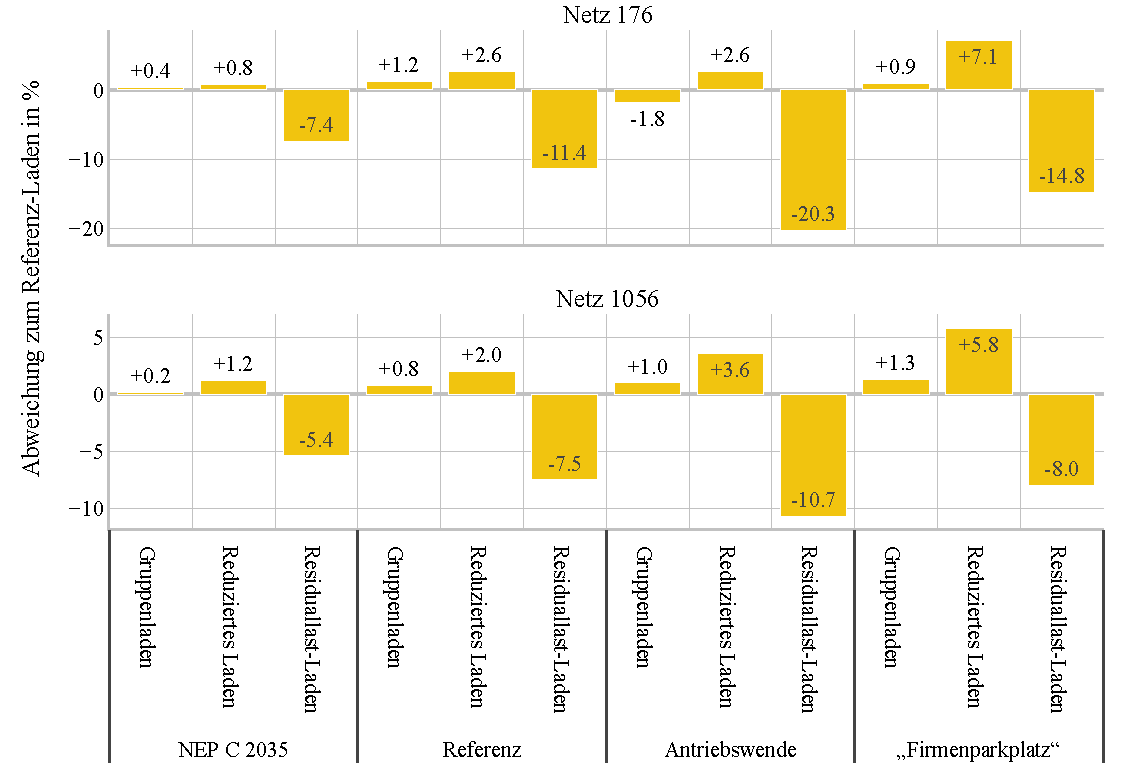
\includegraphics[width=\textwidth]{Bilder/176_1056_cur_fee_grid_week_A}
    \caption{Prozentuale Veränderung des Abregelungsbedarf von fEE Anlagen in Abhängigkeit von der Ladestrategie in Woche A gegenüber dem Abregelungsbedarf für die Referenz-Ladestrategie je Szenario für die Netze \num{176} (oben) und \num{1056} (unten)}\label{fig:176_1056_cur_fee_grid_week_A}
\end{figure}

In \autoref{fig:1056_fEE_load_diff} findet sich die durchschnittliche Abregelung von \gls{FEE} Anlagen und Lasten in Abhängigkeit von der Uhrzeit in Woche~A für das Referenz-Laden im Netz \num{1056}.
Zusätzlich ist die Differenz zwischen den Ladestrategien und dem Referenz-Laden dargestellt, wobei negative Werte einen geringeren Abregelungsbedarf signalisieren.
Dabei zeigt sich, dass in dem stark \gls{PV}-dominierten Netz \num{1056} Abregelung von \gls{FEE} Anlagen ausschließlich tagsüber und vor allem am frühen Nachmittag nötig ist.
Demgegenüber treten die Lastspitzen hierzu versetzt morgens und abends auf.
Durch die Residuallast-Ladestrategie kann der Abregelungsbedarf von \gls{FEE} Anlagen vor allem in Zeiten von Spitzeneinspeisung gesenkt werden.
Beim Gruppenladen und beim reduzierten Laden kommt es zu einem erhöhten Abregelunsgebedarf von \gls{FEE} Anlagen zur Mittagszeit.
Nach \autoref{fig:example_load_profile} werden ab der Mittagszeit viele Fahrzeuge \zH geladen.
Durch die Ladestrategien kommt es dazu, dass der Ladebedarf für den \UC \zH zu dieser Zeit im Durchschnitt geringer ausfällt als beim Referenz-Ladens.
Die Residuallast sinkt somit in Zeiten von Spitzeneinspeisung aufgrund der präventiven Ladestrategien weiter ab, welches den Abregelungsbedarf erhöht und auch in \autoref{fig:residual_load} zu erkennen ist.


\begin{figure}[H]
    \centering
    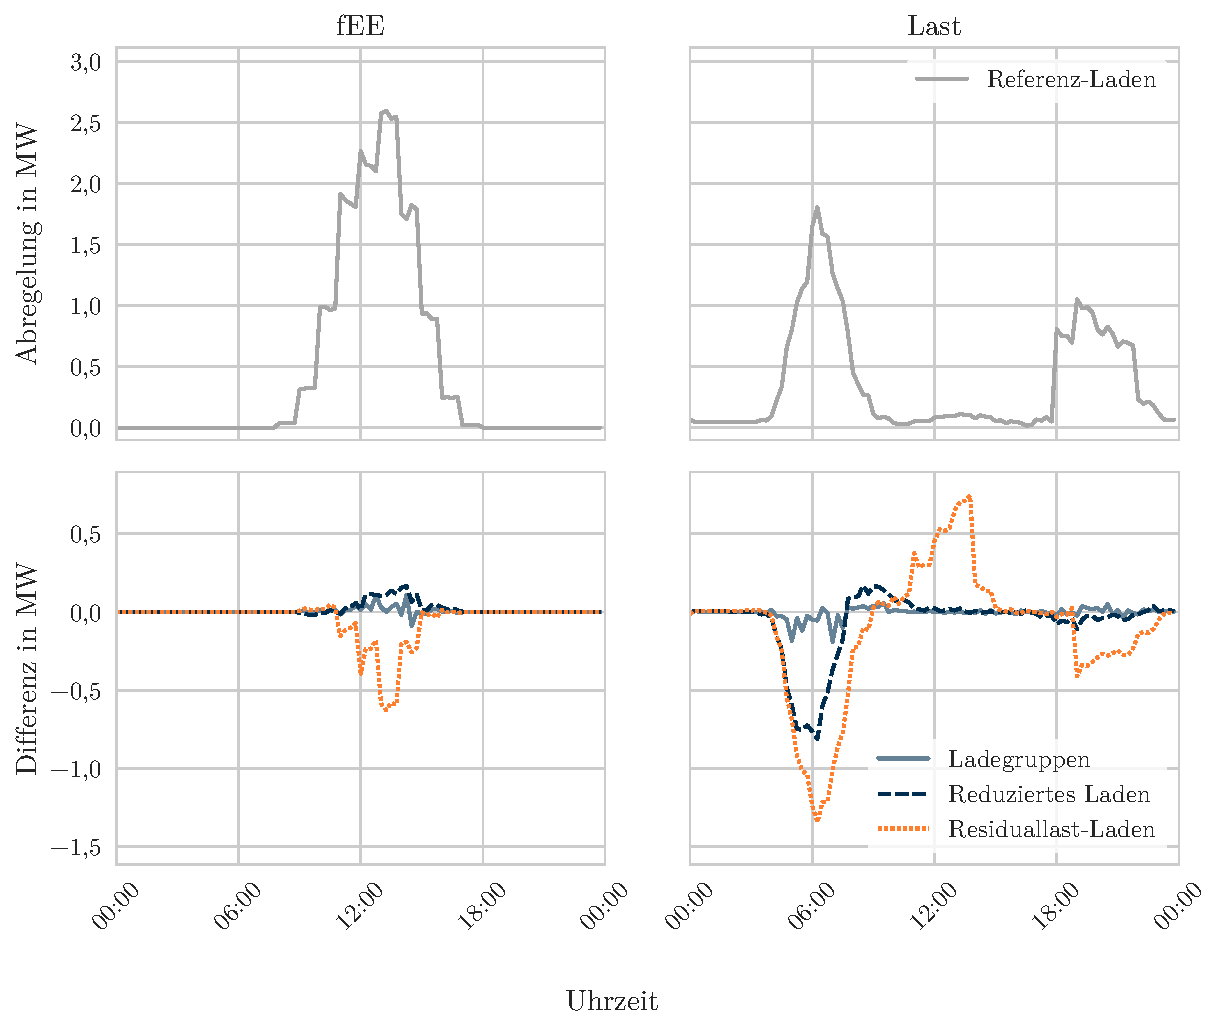
\includegraphics[width=\textwidth]{Bilder/1056_fEE_load_diff}
    \caption{Durchschnittliche Abregelung von fEE Anlagen (oben links) und Lasten (oben rechts) innerhalb von Woche A und die durchschnittliche Differenz des Abregelungsbedarfs der Ladestrategien gegenüber dem Referenz-Laden für fEE Anlagen (unten links) und Lasten (unten rechts) im Antriebswende-Szenario im Netz \num{1056}}\label{fig:1056_fEE_load_diff}
\end{figure}

Lastseitig können sowohl durch die Residuallast-Ladestrategie als auch durch das reduzierte Laden in erster Linie morgens große Mengen an Abregelung verhindert werden.
Zusätzlich kann durch die Residuallast-Ladestrategie auch am Abend ein signifikanter Anteil an Abregelung vermieden werden.
Zur Mittagszeit zeigt sich lastseitig ein erhöhter Abregelungsbedarf durch die Residuallast-Ladestrategie.
Es wird somit ein zu großer Anteil von Fahrzeugen innerhalb eines kurzen Zeitfensters geladen und vor allem die Betriebsmittel auf der \gls{NS}-Ebene überlastet.


\paragraph{Fazit:}

Der Hochlauf der Elektromobilität gestaltet sich in den beiden betrachteten \gls{PV}-dominierten Netzen stark unterschiedlich.
Im Falle des Netzes \num{176} werden einzelne \gls{NS}-Netze so stark überlastet, dass ein großer Anteil des Ladebedarfs der \gls{EPKW} abgeregelt werden muss.
Demgegenüber fällt der Abregelungsbedarf des Ladebedarfs im Netz \num{1056} deutlich moderater aus. \medskip

Das Gruppenladen zeigt insgesamt eine sehr geringe Wirksamkeit auf den Abregelungsbedarf.
Für die anderen Ladestrategien ergeben sich aus der unterschiedlich starken Überlastung der beiden Netze starke Potentialunterschiede in der Wirksamkeit.
So kann das reduzierte Laden weitgehend den lastseitigen Abregelungsbedarf um einen signifikanten Anteil senken.
Dabei zeigt sich jedoch, dass das Einsparpotential mit einer zunehmenden Überlastung der \gls{NS}-Netze abnimmt, da es zunehmend auch Nachts zu Abregelungen des Ladebedarfs kommt und dieser zeitlich nur noch verschoben aber nicht verhindert wird.
Das aktive Residuallast-Laden kann gegenüber den präventiven Ladestrategien weitere lastseitige Abregelung verhindern, wenn die entsprechenden \gls{NS}-Netzkapazitäten gegeben sind oder die Erzeugerkapazitäten in den gleichen \gls{NS}-Netzen liegen, in denen auch der Ladebedarf anfällt.\medskip

Es zeigt sich, dass nur durch die aktive Verschiebung des Ladebedarfs in die Hochzeiten der Einspeisung von \gls{FEE} Anlagen bei der Residuallast-Ladestrategie der erzeugerseitige Abregelungsbedarf reduziert werden kann.
Allerdings wird in der Regel so viel Ladebedarf in die Hochzeiten der Einspeisung verschoben, dass es aufgrund der hohen Gleichzeitigkeit zu einer erhöhten Abregelung des Ladebedarfs kommt.
Das Potential den lastseitigen und erzeugerseitigen Abregelungsbedarf zu senken, wird auf diese Weise nicht voll ausgeschöpft.
Es empfiehlt sich neben dem Optimierungsansatz der Residuallast-Glättung vor allem auch die Belastungsgrenzen der \gls{NS}-Betriebsmittel zu beachten.
Auf diese Weise würde mehr Ladebedarf in Zeiten einer schwächeren Einspeisung verschoben werden und voraussichtlich könnte der Abregelungsbedarf last- und einspeiseseitig weiter gesenkt werden.
Die präventiven Ladestrategie führen demgegenüber zu einer Erhöhung des erzeugerseitigen Abregelungsbedarfs, da der Ladebedarf am frühen Nachmittag reduziert wird und somit nicht mehr in die Hochzeiten der Einspeisung der \gls{FEE} Anlagen fällt.


\subsubsection{Wind-dominierte Netze}

Die Wind-dominierten Netze \num{1690} und \num{1811} weisen gegenüber den \gls{PV}-dominierten Netzen eine deutlich größere Differenz zwischen Erzeugung und Bedarf auf.
So liegt das Verhältnis zwischen der Einspeisung von \gls{FEE} Anlagen und dem Ladebedarf von \gls{EPKW} nach \autoref{tab:wind_dominated_week_a_char} und \autoref{tab:wind_dominated_epkw_demand} im Antriebswende-Szenario in Woche~A im Netz \num{1811} bei etwa \(19:1\) und im Netz \num{1690} sogar bei etwa \(33:1\).
Hieraus folgt gegenüber den \gls{PV}-dominierten Netzen ein deutlich reduziertes Potential den Abregelungsbedarf von \gls{FEE} Anlagen zu beeinflussen.


{
\renewcommand{\arraystretch}{1.2}% grßerer Zeilenabstand
\sisetup{range-phrase=~{--}~}% Gedankenstrich statt "bis" bei SIrange
\begin{table}[H]
	\begin{center}
		\caption{Einspeisung von fEE und nicht-fEE Anlagen sowie der Bedarf von sonstigen Lasten in den Wind-dominierten Netzen}
		\begin{tabu} to 0.7\textwidth {X[2] X[1, r] X[1, r]}
			\toprule
											  & Netz \num{1690} & Netz \num{1811} \\ \midrule
			Einspeisung fEE in \si{\mwh}      & \num{11971.2}   & \num{8966.5}    \\
			Einspeisung Sonstige in \si{\mwh} & \num{4808.5}    & \num{2541.0}    \\
			Bedarf Sonstige  in \si{\mwh}     & \num{1442.8}    & \num{1599.2}    \\ \bottomrule
		\end{tabu}
		\label{tab:wind_dominated_week_a_char}
	\end{center}
	\vspace{-3mm}%Put here to reduce too much white space after your table
\end{table}
}

{
\renewcommand{\arraystretch}{1.2}% grßerer Zeilenabstand
\sisetup{range-phrase=~{--}~}% Gedankenstrich statt "bis" bei SIrange
\begin{table}[H]
	\begin{center}
		\caption{Ladebedarf der E-Pkw in den Wind-dominierten Netzen je Szenario}
		\begin{tabu} to 0.6\textwidth {X[1.5] X[1, r] X[1, r]}
			\toprule
			Ladebedarf in   \si{\mwh}    & Netz \num{1690} & Netz \num{1811} \\ \midrule
			NEP C~\num{2035}             & \num{111.9}     & \num{135.2}     \\
			Referenz                     & \num{199.2}     & \num{244.6}     \\
			Antriebswende                & \num{361.5}     & \num{465.3}     \\
			\glqq Firmenparkplatz\grqq{} & \num{363.0}     & \num{459.9}     \\ \bottomrule
		\end{tabu}
		\label{tab:wind_dominated_epkw_demand}
	\end{center}
	\vspace{-3mm}%Put here to reduce too much white space after your table
\end{table}
}

In \autoref{tab:wind_dominated_week_a_epkw_cur} findet sich der Abregelungsbedarf des Ladebedarfs von \gls{EPKW} in den Wind-dominierten Netzen für die Referenz-Ladestrategie in Woche~A und in \autoref{tab:wind_dominated_week_a_load_cur} ergänzend der Abregelungsbedarf für die sonstigen Lasten.
Auch bei den Wind-dominierten Netzen kommt es zu einer Zunahme des Abregelungsbedarf mit dem Hochlauf der \gls{EPKW}.
Da die Windkraft-Erzeugerkapazitäten in der Regel direkt in der \gls{MS}-Ebene angeschlossen werden und auch absolut eine größer Erzeugerleistung in den den Wind-dominierten Netzen installiert ist (vgl. \autoref{fig:bar_representatives}), ist die \gls{MS}-Ebene in den Wind-dominierten Netzen auf höhere Lasten ausgelegt als in den \gls{PV}-dominierten Netzen.
Der lastseitige Abregelungsbedarf beschränkt sich deshalb beinahe vollständig auf die \gls{NS}-Ebene.
Das Netz \num{1690} zeigt im Gegensatz zu den anderen Netzen einen höheren Abregelungsbedarf in der \SzeFirmenparkplatz gegenüber dem Antriebswende-Szenario.
Hierbei kommt es zu dem Effekt, dass die zusätzliche Abregelung am Nachmittag und Abend aufgrund des höheren Anteils an öffentlicher Ladeinfrastruktur und von Ladeinfrastruktur zu Hause größer ausfällt als die Abregelungseinsparung am Morgen durch den geringeren Anteil an Ladeinfrastruktur auf Firmenparkplätzen.
Auch fällt in dem Netz \num{1690} der Ladebedarf in der \SzeFirmenparkplatz leicht höher aus als im Antriebswende-Szenario.

{
\renewcommand{\arraystretch}{1.2}% grßerer Zeilenabstand
\sisetup{range-phrase=~{--}~}% Gedankenstrich statt "bis" bei SIrange
\begin{table}[H]
	\begin{center}
		\caption{Abregelungsbedarf des Ladebedarfs von E-Pkw in den Wind-dominierten Netzen je Szenario für die Referenz-Ladestrategie in Woche A}
		\begin{tabu} to 0.6\textwidth {X[1.5] X[1, r] X[1, r]}
			\toprule
			Abregelung in   \si{\mwh}    & Netz \num{1690} & Netz \num{1811} \\ \midrule
			NEP C~\num{2035}             & \num{2.5}       & \num{1.6}       \\
			Referenz                     & \num{7.8}       & \num{7.1}       \\
			Antriebswende                & \num{18.4}      & \num{20.4}      \\
			\glqq Firmenparkplatz\grqq{} & \num{20.1}      & \num{17.7}      \\ \bottomrule
		\end{tabu}
		\label{tab:wind_dominated_week_a_epkw_cur}
	\end{center}
	\vspace{-3mm}%Put here to reduce too much white space after your table
\end{table}
}

{
\renewcommand{\arraystretch}{1.2}% grßerer Zeilenabstand
\sisetup{range-phrase=~{--}~}% Gedankenstrich statt "bis" bei SIrange
\begin{table}[H]
	\begin{center}
		\caption{Abregelungsbedarf der sonstigen Lasten in den Wind-dominierten Netzen je Szenario für die Referenz-Ladestrategie in Woche A}
		\begin{tabu} to 0.6\textwidth {X[1.5] X[1, r] X[1, r]}
			\toprule
			Abregelung in   \si{\mwh}    & Netz \num{1690} & Netz \num{1811} \\ \midrule
			NEP C~\num{2035}             & \num{3.5}       & \num{2.6}       \\
			Referenz                     & \num{4.4}       & \num{3.7}       \\
			Antriebswende                & \num{7.0}       & \num{6.3}       \\
			\glqq Firmenparkplatz\grqq{} & \num{7.0}       & \num{6.3}       \\ \bottomrule
		\end{tabu}
		\label{tab:wind_dominated_week_a_load_cur}
	\end{center}
	\vspace{-3mm}%Put here to reduce too much white space after your table
\end{table}
}

In den Wind-dominierten Netzen kann der lastseitige Abregelungsbedarf nach \autoref{fig:1690_1811_cur_load_grid_week_A} und \autoref{fig:1690_1811_cur_load_grid_week_B} in beinahe allen Fällen durch die Ladestrategien gesenkt werden.
Es zeigt sich erneut, dass das Gruppenladen nur einen geringen Einfluss auf den lastseitigen Abregelungsbedarf aufweist.
Das reduzierte Laden erweist sich im Gegensatz zu den \gls{PV}-dominierten Netzen in allen Fällen effektiver als das Residuallast-Laden, um den lastseitigen Abregelungsbedarf zu senken.\medskip

In Woche~A kann im Netz \num{1811} durch das reduzierte Laden noch eine annährend konstante Senkungswirkung der lastseitigen Abregelung in den unterschiedlichen Szenarien erreicht werden.
Demgegenüber kann in Woche~B und und im Netz \num{1690} eine Abnahme des Einsparpotentials an lastseitiger Abregelung mit einem zunehmenden Hochlauf an \gls{EPKW} festgestellt werden.

\begin{figure}[H]
    \centering
    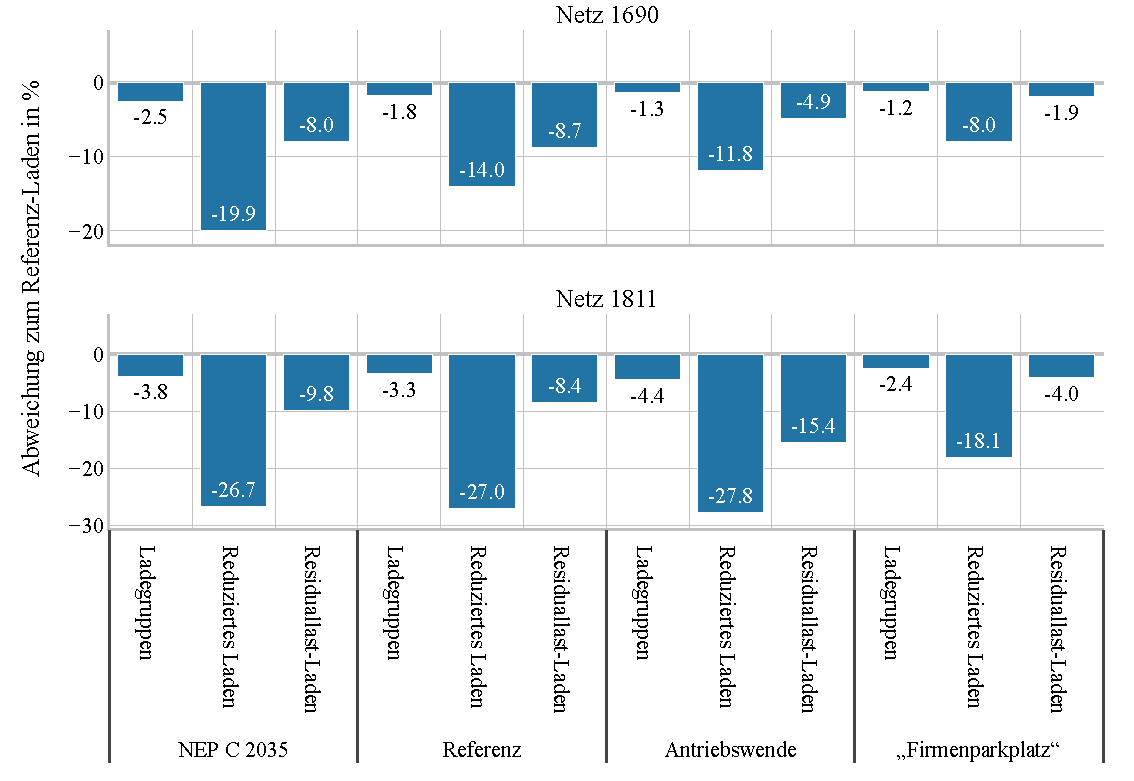
\includegraphics[width=\textwidth]{Bilder/1690_1811_cur_load_grid_week_A}
    \caption[Prozentuale Veränderung des Abregelungsbedarfs von allen Lasten in Abhängigkeit von der Ladestrategie in Woche~MIN gegenüber dem Abregelungsbedarf für die Referenz-Ladestrategie je Szenario für die Netze \num{1690} und \num{1811}]{Prozentuale Veränderung des Abregelungsbedarfs von allen Lasten in Abhängigkeit von der Ladestrategie in Woche~MIN gegenüber dem Abregelungsbedarf für die Referenz-Ladestrategie je Szenario für die Netze \(1690_{\text{W}}\) (oben) und \(1811_{\text{W}}\) (unten)}\label{fig:1690_1811_cur_load_grid_week_A}
\end{figure}

Der Trend hin zu einem sinkenden prozentualem Einsparpotential durch das reduzierte Laden tritt im Netz \num{1690} in beiden Wochen auf und im Netz \num{1811} nur in Woche~B.
Die beiden Netze Verhalten sich hierbei ähnlich wie das \gls{PV}-dominierte Netz \num{176}.
Im Unterschied zu dem Netz \num{176} kommt es in den Wind-dominierten Netzen nachts in der Regel nicht zu einer lastseitigen Abregelung (vgl. \autoref{fig:1690_fEE_load_diff} (oben rechts)).
Hierdurch kann durch das reduzierte Laden in allen Fällen Ladebedarf in die Nacht verschoben werden, ohne nachts zu einem erhöhten Abregelungsbedarf zu führen, weshalb die Einsparpotentiale im Gegensatz zum Netz \num{176} höher ausfallen.
In den Szenarien mit einem geringeren Hochlauf an \gls{EPKW} kommt es beim Referenz-Laden in erster Linie zur Abregelung von Last am Morgen und am Abend.
Bei einem höheren Hochlauf an \gls{EPKW} kommt es zusätzlich zur lastseitigen Abregelungen zur Mittagszeit und am frühen Nachmittag.
Durch das reduzierte Laden kann in diesen Fällen Abregelungsbedarf nur mit nachlassendem Erfolg verhindert werden, da vermehrt Abregelungsbedarf nur noch vom Vormittag auf den frühen Nachmittag verschoben wird.
Das Netz \num{1811} besitzt bei einem moderat erhöhtem Ladebedarf gegenüber dem Netz \num{1690} eine deutlich höhere Anzahl an \gls{NS}-Netzen weshalb die einzelnen \gls{NS}-Netze meist geringer belastet werden.
Hierdurch kommt es zu diesem Trend im Netz \num{1811} erst in dem erhöhten Lastfällen der Woche~B.

\begin{figure}[H]
    \centering
    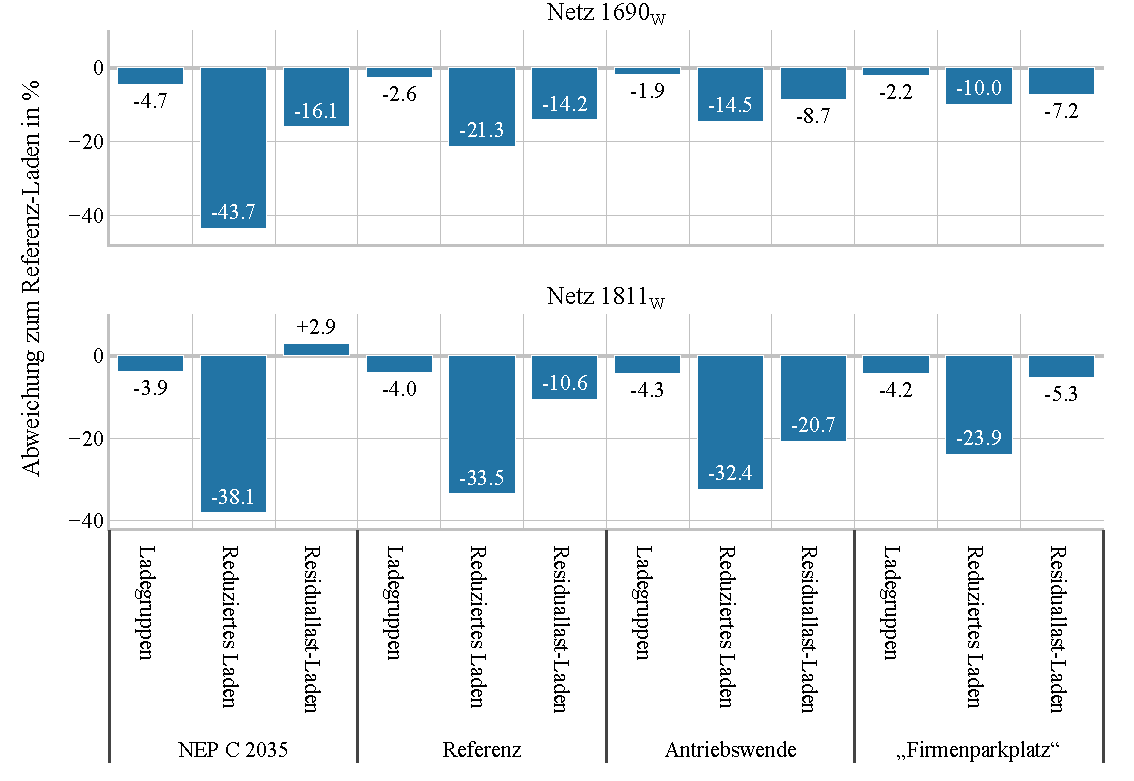
\includegraphics[width=\textwidth]{Bilder/1690_1811_cur_load_grid_week_B}
    \caption[Prozentuale Veränderung des Abregelungsbedarfs von allen Lasten in Abhängigkeit von der Ladestrategie in Woche~MAX gegenüber dem Abregelungsbedarf für die Referenz-Ladestrategie je Szenario für die Netze \num{1690} und \num{1811}]{Prozentuale Veränderung des Abregelungsbedarfs von allen Lasten in Abhängigkeit von der Ladestrategie in Woche~MAX gegenüber dem Abregelungsbedarf für die Referenz-Ladestrategie je Szenario für die Netze \(1690_{\text{W}}\) (oben) und \(1811_{\text{W}}\) (unten)}\label{fig:1690_1811_cur_load_grid_week_B}
\end{figure}

Der Vorteil des reduzierten Ladens gegenüber dem Residuallast-Laden entsteht, weil es auch in den Wind-dominierten Netzen einen gewissen Anteil an \gls{PV}-Erzeugerkapazitäten gibt.
Dies führt dazu, dass beim Residuallast-Laden ein großer Anteil an Ladevorgängen in die Hochzeit der \gls{PV}-Einspeisung zum Mittag und frühen Nachmittag verschoben wird.
Da die \gls{NS}-Netze in diesem Zeitraum bereits stark belastet sind, führt diese zusätzliche Last zu einem erhöhten Abregelungsbedarf, welches in \autoref{fig:1690_fEE_load_diff} (unten rechts) zu erkennen ist.
Weiterhin ist aufgrund des hohen Verhältnisses zwischen Einspeisung und Ladebedarf in den Wind-dominierten Netzen der Einfluss des Ladebedarfs auf die Residuallast gering.
Hierdurch tritt eine besonders starke temporäre Konzentration der Ladevorgänge in den Wind-dominierten Netzen beim Residuallast-Laden auf, was den Abregelungsbedarf weiter erhöht.

{
\renewcommand{\arraystretch}{1.2}% grßerer Zeilenabstand
\sisetup{range-phrase=~{--}~}% Gedankenstrich statt "bis" bei SIrange
\begin{table}[H]
	\begin{center}
		\caption{Abregelungsbedarf von fEE Anlagen in den Wind-dominierten Netzen je Szenario für die Referenz-Ladestrategie in Woche A}
		\begin{tabu} to 0.6\textwidth {X[1.5] X[1, r] X[1, r]}
			\toprule
			Abregelung in   \si{\mwh}    & Netz \num{1690} & Netz \num{1811} \\ \midrule
			NEP C~\num{2035}             & \num{319.1}     & \num{0.0}       \\
			Referenz                     & \num{315.2}     & \num{0.0}       \\
			Antriebswende                & \num{312.3}     & \num{0.0}       \\
			\glqq Firmenparkplatz\grqq{} & \num{311.9}     & \num{0.0}       \\ \bottomrule
		\end{tabu}
		\label{tab:wind_dominated_week_a_fee_cur}
	\end{center}
	\vspace{-3mm}%Put here to reduce too much white space after your table
\end{table}
}

Bei der Abregelung von \gls{FEE} Anlagen in den Wind-dominierten Netzen zeigt sich, dass keine Abregelung in Woche~B nötig ist.
Weiterhin ist im Netz \num{1811} nach \autoref{tab:wind_dominated_week_a_fee_cur} auch in Woche~A keine Abregelung notwendig, weshalb der Fokus auf der Betrachtungen der Woche~A im Netz \num{1690} liegt.
Im Netz \num{1690} zeigt sich vergleichbar zu den \gls{PV}dominierten eine Abnahme des Abregelungsbedarfs mit dem Hochlauf an \gls{EPKW}.\medskip

Die Ladestrategien zeigen nach \autoref{fig:1690_cur_fee_grid_week_A} insgesamt einen extrem geringen Einfluss auf den erzeugungsseitigen Abregelungsbedarf von maximal \SI{1}{\percent}.
Dies liegt zum einen darin begründet, dass das Verhältnis aus Erzeugung zu Ladebedarf im Netz \num{1690} extrem hoch ausfällt und zum anderen darin, dass in Woche~A in \SI{83}{\percent} der Zeitschritte eine erzeugerseitige Abregelung nötig ist, welches sich in \autoref{fig:1690_fEE_load_diff} darin äußert, dass die durchschnittliche Abregelung der \gls{FEE} Anlagen (oben links) nie auf Null sinkt.
Hierdurch ergibt sich auf der einen Seite, dass das Potential zur Einflussnahme sehr gering ausfällt und auf der anderen Seite, dass auch erzeugerseitige Abregelung nur zeitlich verschoben wird.
So wird beispielsweise beim reduzierten Laden vor allem nachts Abregelung von Windkraftanlagen verhindert.
Dafür kommt es morgens und nachmittags zu einem erhöhten Abregelungsbedarf, da der Ladebedarf in diesen Zeitfenstern stark reduziert wird.
Insgesamt wird der Abregelungsbedarf hierdurch leicht erhöht.

\begin{figure}[H]
    \centering
    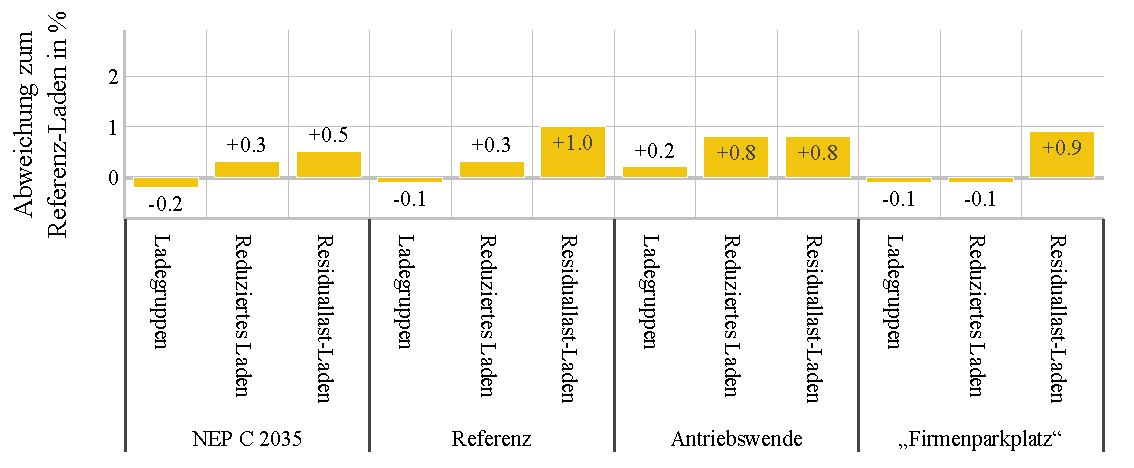
\includegraphics[width=\textwidth]{Bilder/1690_cur_fee_grid_week_A}
    \caption[Prozentuale Veränderung des Abregelungsbedarfs von fEE Anlagen in Abhängigkeit von der Ladestrategie in Woche~MIN gegenüber dem Abregelungsbedarf für die Referenz-Ladestrategie je Szenario für das Netze \num{1690}]{Prozentuale Veränderung des Abregelungsbedarfs von fEE Anlagen in Abhängigkeit von der Ladestrategie in Woche~MIN gegenüber dem Abregelungsbedarf für die Referenz-Ladestrategie je Szenario für das Netze \(1690_{\text{W}}\)}\label{fig:1690_cur_fee_grid_week_A}
\end{figure}

Im Gegensatz zu den \gls{PV}-dominierten Netzen zeigt sich, dass der erzeugerseitige Abregelungsbedarf durch die Residuallast-Ladestrategie nicht abgesenkt werden kann und sich sogar deutlicher erhöht als bei den präventiven Ladestrategien.
Hierbei kommt es zu einer ungünstigen temporalen und lokalen Konzentration von Ladevorgängen.
So kann der erzeugerseitige Abregelungsbedarf nach \autoref{fig:1690_fEE_load_diff} am frühen Nachmittag (grüner Bereich) gesenkt werden, während sich der Abregelungsbedarf anschließend (roter Bereich) erhöht.
In dem grünen Bereich kommt es in erster Linie zu einer Anhebung des Ladebedafs von Fahrzeugen auf Firmenparkplätzen, da zu dieser Zeit aufgrund des \gls{PV}-Anteils im \gls{MS}-Netz in der Regel die geringste Residuallast während der üblichen Standzeiten auf Firmenparkplätzen vorherscht.
Weiterhin sind die Standzeiten auf Firmenparkplätzen in der Regel kürzer als zu Hause (vgl. \autoref{tab:StandingTime}), weshalb die Priorität dieser Ladevorgänge bei der Vergabe der Ladezeitfenster nach \autoref{chap:theo_strategies} erhöht wird.
Innerhalb der \gls{NS}-Netze in denen viele Ladevorgänge auf Firmenparkplätzen stattfinden, befinden sich im Netz \num{1690} nur wenige \glspl{PVA}.
Aus diesem Grund kommt es zwar insgesamt zu einer Reduktion des erzeugerseitigen Abregelungsbedarfs, aber dieser fällt im Verhältnis zum aufgewendeten Ladebedarf gering aus.
Zusätzlich erhöht sich in diesem Zeitfenster der Abregelungsbedarf der Lasten was die Effizienz der Ladestrategie weiter senkt.

\begin{figure}[H]
    \centering
    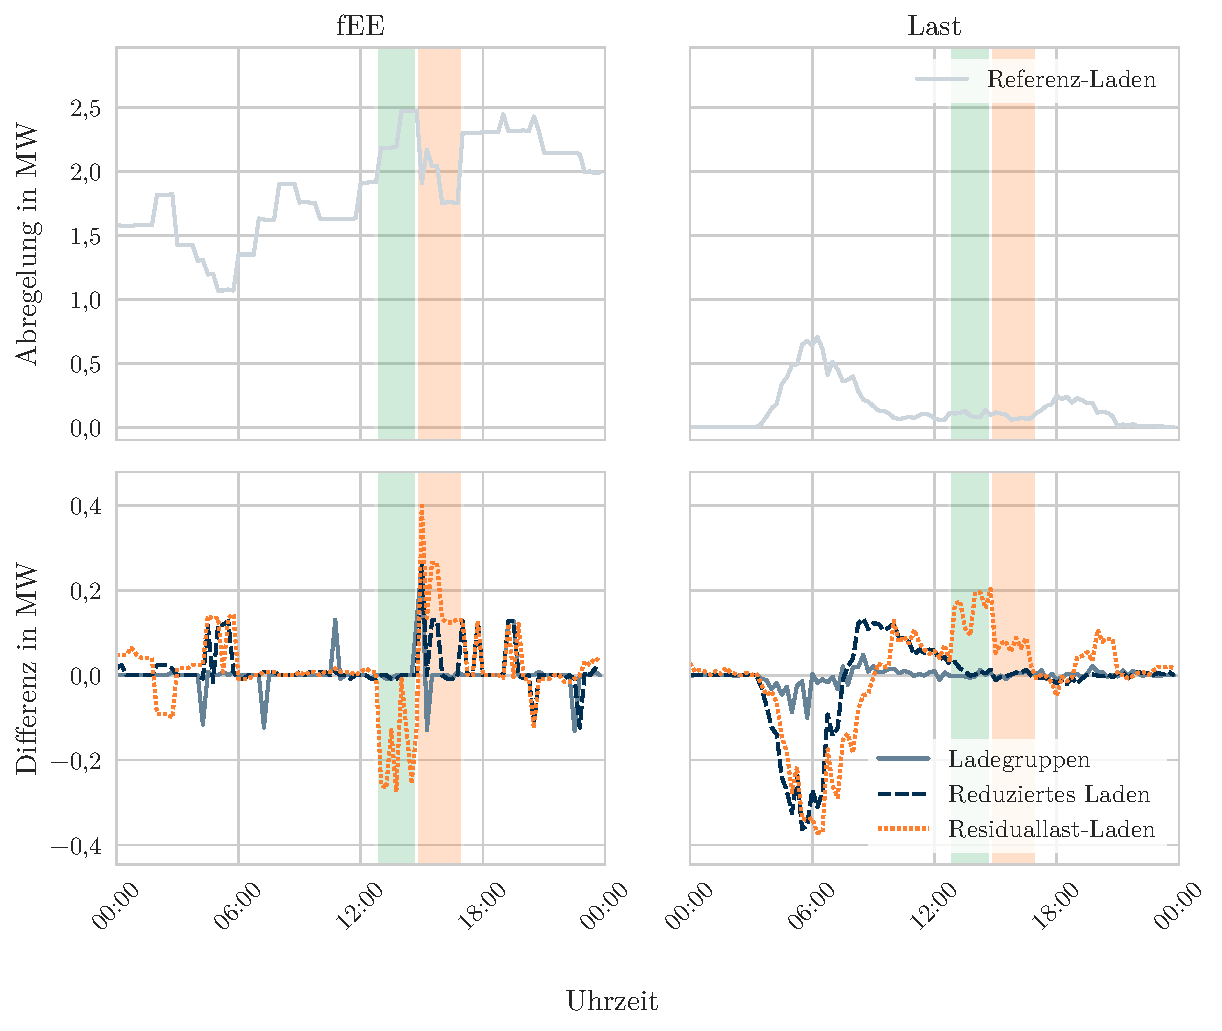
\includegraphics[width=\textwidth]{Bilder/1690_fEE_load_diff}
    \caption{Durchschnittliche Abregelung von fEE Anlagen (oben links) und Lasten (oben rechts) innerhalb von Woche~MIN und die durchschnittliche Differenz des Abregelungsbedarfs der Ladestrategien gegenüber dem Referenz-Laden für fEE Anlagen (unten links) und Lasten (unten rechts) im Antriebswende-Szenario im Netz \num{1690}}\label{fig:1690_fEE_load_diff}
\end{figure}

Im roten Bereich kommt es ebenfalls zu einem erhöhten Ladebedarf von Fahrzeugen auf Firmenparkplätzen.
Diese Erhöhung fällt jedoch geringer aus als im grünen Bereich und der lastseitigen Abregelungsbedarf wird entsprechend weniger stark erhöht.
Gleichzeitig wird der Ladebedarf zu Hause gegenüber der Referenz-Ladestrategie abgesenkt, da die Residuallast in der Regel nachts niedriger ausfällt und die Ladevorgänge zu Hause somit vermehrt nachts stattfinden.
Innerhalb der \gls{NS}-Netze in denen primär Ladevorgänge zu Hause stattfinden, befinden sich im \gls{MS}-Netz \num{1690} viele \glspl{PVA}.
Hierdurch erhöht sich sowohl der erzeugerseitige \gls{NS}- als auch \gls{MS}-Abregelungsbedarf.
Windkraftanlagen befinden sich demgegenüber nicht in der örtlichen Nähe der \gls{NS}-Netze in denen primär Ladevorgänge zu Hause stattfinden.
Da es jedoch nachts ausschließlich zu Abregelungen von Windkraftanlagen kommt, wird der nächtliche Abregelungsbedarf durch die Ladevorgänge kaum beeinflusst.



\paragraph{Fazit:}

In den Wind-dominierten Netzen kommt es lastseitig vor allem zu Abregelungen auf der \gls{NS}-Ebene, da die \gls{MS}-Ebene in der Regel gut ausgebaut ist.
Erzeugerseitige Abregelung findet nur im Netz \num{1690} statt.\medskip

Auch bei den Wind-domninierten Netzen zeigt sich das Gruppenladen als weitgehend ineffektiv und kann den lastseitigen Abregelungsbedarf nur leicht reduzieren.
Das reduzierte Laden kann hingegen in der Regel einen großen Anteil des lastseitigen Abregelungsbedarfs verhindern, wobei sich bestätigt, dass das Einsparpotential mit einer zunehmenden Belastung der \gls{NS}-Netze abnimmt.
Das aktive Residuallast-Laden erweist sich lastseitig in den Wind-dominierten Netzen als weniger effektiv als das reduzierte Laden.
Aufgrund des hohen Verhältnisses zwischen Einspeisung und Ladebedarf kommt es beim Residuallast-Laden zu einer hohen Konzentration des Ladebedarfs auf wenige Zeitschritte.
Hierdurch kann der lastseitige Abregelungsbedarf, trotz einer starken Reduktion am Morgen, insgesamt nur leicht gesenkt werden, da der Abregelungsbedarf am Nachmittag stark zunimmt.\medskip

Der Abregelungsbedarf von \gls{FEE} Anlagen kann durch die untersuchten Ladestrategien zum einen nur in einem sehr geringen Maße und zum anderen nicht positiv beeinflusst werden.
So richtet sich das Residuallast-Laden nach einer globalen Residuallast im \gls{MS}-Netz die keine lokalen Unterschiede im \gls{MS}-Netz beachtet.
So werden Ladevorgänge zwar zeitlich in günstige Zeitfenster verschoben, aber diese finden an ungünstigen Lokalitäten statt, wodurch sich der Abregelungsbedarf sogar weiter erhöht.
Es empfiehlt sich somit, die lokale Netztopologie mit in die Priorisierung der Ladevorgänge mit einzubeziehen, um eine ungünstige lokale Verteilung der Ladevorgänge zu vermeiden.


\subsubsection{Das Last-dominierte Netz}

{
\renewcommand{\arraystretch}{1.2}% grßerer Zeilenabstand
\sisetup{range-phrase=~{--}~}% Gedankenstrich statt "bis" bei SIrange
\begin{table}[H]
	\begin{center}
		\caption{Einspeisung von fEE und nicht-fEE Anlagen sowie der Bedarf von sonstigen Lasten in dem Last-dominierten Netz}
		\begin{tabu} to 0.7\textwidth {X[2] X[1, r] X[1, r]}
			\toprule
											  & Woche A      & Woche B      \\ \midrule
			Einspeisung fEE in \si{\mwh}      & \num{871.5}  & \num{51.8}   \\
			Einspeisung Sonstige in \si{\mwh} & \num{47.2}   & \num{47.2}   \\
			Bedarf Sonstige  in \si{\mwh}     & \num{5413.0} & \num{5716.0} \\ \bottomrule
		\end{tabu}
		\label{tab:load_dominated_char}
	\end{center}
	\vspace{-3mm}%Put here to reduce too much white space after your table
\end{table}
}

\autoref{tab:load_dominated_char}

{
\renewcommand{\arraystretch}{1.2}% grßerer Zeilenabstand
\sisetup{range-phrase=~{--}~}% Gedankenstrich statt "bis" bei SIrange
\begin{table}[H]
	\begin{center}
		\caption{Ladebedarf der E-Pkw in dem Last-dominierten Netz je Szenario}
		\begin{tabu} to 0.6\textwidth {X[1.5] X[1, r] X[1, r]}
			\toprule
			Ladebedarf in   \si{\mwh}    & Woche A     & Woche B     \\ \midrule
			NEP C~\num{2035}             & \num{271.3} & \num{271.3} \\
			Referenz                     & \num{485.3} & \num{485.3} \\
			Antriebswende                & \num{919.0} & \num{919.0} \\
			\glqq Firmenparkplatz\grqq{} & \num{915.3} & \num{915.3} \\ \bottomrule
		\end{tabu}
		\label{tab:load_dominated_epkw_demand}
	\end{center}
	\vspace{-3mm}%Put here to reduce too much white space after your table
\end{table}
}

\autoref{tab:load_dominated_epkw_demand}

{
\renewcommand{\arraystretch}{1.2}% grßerer Zeilenabstand
\sisetup{range-phrase=~{--}~}% Gedankenstrich statt "bis" bei SIrange
\begin{table}[H]
	\begin{center}
		\caption{Abregelungsbedarf des Ladebedarfs von E-Pkw in dem Last-dominierten Netz je Szenario für die Referenz-Ladestrategie}
		\begin{tabu} to 0.6\textwidth {X[1.5] X[1, r] X[1, r]}
			\toprule
			Abregelung in   \si{\mwh}    & Woche A     & Woche B     \\ \midrule
			NEP C~\num{2035}             & \num{60.5}  & \num{68.9}  \\
			Referenz                     & \num{147.4} & \num{160.8} \\
			Antriebswende                & \num{337.8} & \num{360.9} \\
			\glqq Firmenparkplatz\grqq{} & \num{381.5} & \num{405.5} \\ \bottomrule
		\end{tabu}
		\label{tab:load_dominated_epkw_cur}
	\end{center}
	\vspace{-3mm}%Put here to reduce too much white space after your table
\end{table}
}

\autoref{tab:load_dominated_epkw_cur}

{
\renewcommand{\arraystretch}{1.2}% grßerer Zeilenabstand
\sisetup{range-phrase=~{--}~}% Gedankenstrich statt "bis" bei SIrange
\begin{table}[H]
	\begin{center}
		\caption{Abregelungsbedarf der sonstigen Lasten im Last-dominierten Netz je Szenario für die Referenz-Ladestrategie}
		\begin{tabu} to 0.6\textwidth {X[1.5] X[1, r] X[1, r]}
			\toprule
			Abregelung in   \si{\mwh}    & Woche A     & Woche B     \\ \midrule
			NEP C~\num{2035}             & \num{179.6} & \num{247.7} \\
			Referenz                     & \num{211.7} & \num{274.3} \\
			Antriebswende                & \num{253.1} & \num{318.5} \\
			\glqq Firmenparkplatz\grqq{} & \num{253.2} & \num{319.5} \\ \bottomrule
		\end{tabu}
		\label{tab:load_dominated_load_cur}
	\end{center}
	\vspace{-3mm}%Put here to reduce too much white space after your table
\end{table}
}

\autoref{tab:load_dominated_load_cur}

\begin{figure}[H]
    \centering
    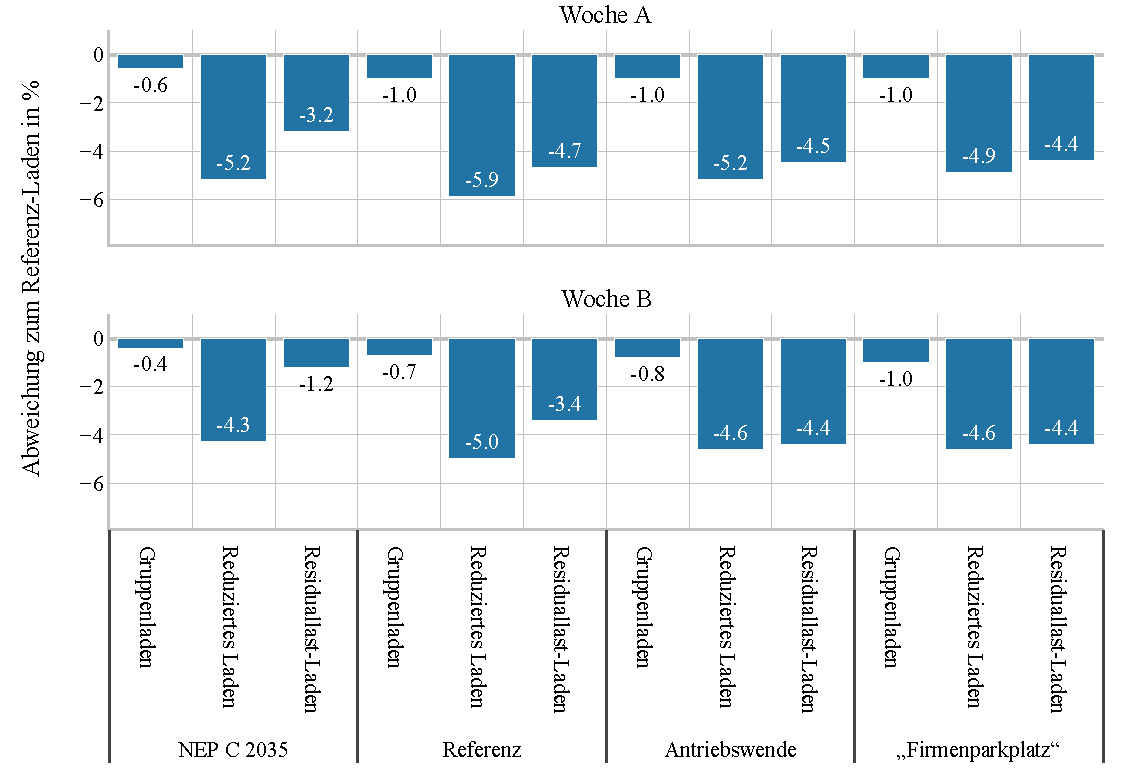
\includegraphics[width=\textwidth]{Bilder/177_cur_load_both_weeks}
    \caption{Prozentuale Veränderung des Abregelungsbedarfs von allen Lasten in Abhängigkeit von der Ladestrategie in Woche~A (oben) und Woche~B (unten) gegenüber dem Abregelungsbedarf für die Referenz-Ladestrategie je Szenario für das Netz \num{177}}\label{fig:177_cur_load_both_weeks}
\end{figure}

\autoref{fig:177_cur_load_both_weeks}

\begin{figure}[H]
    \centering
    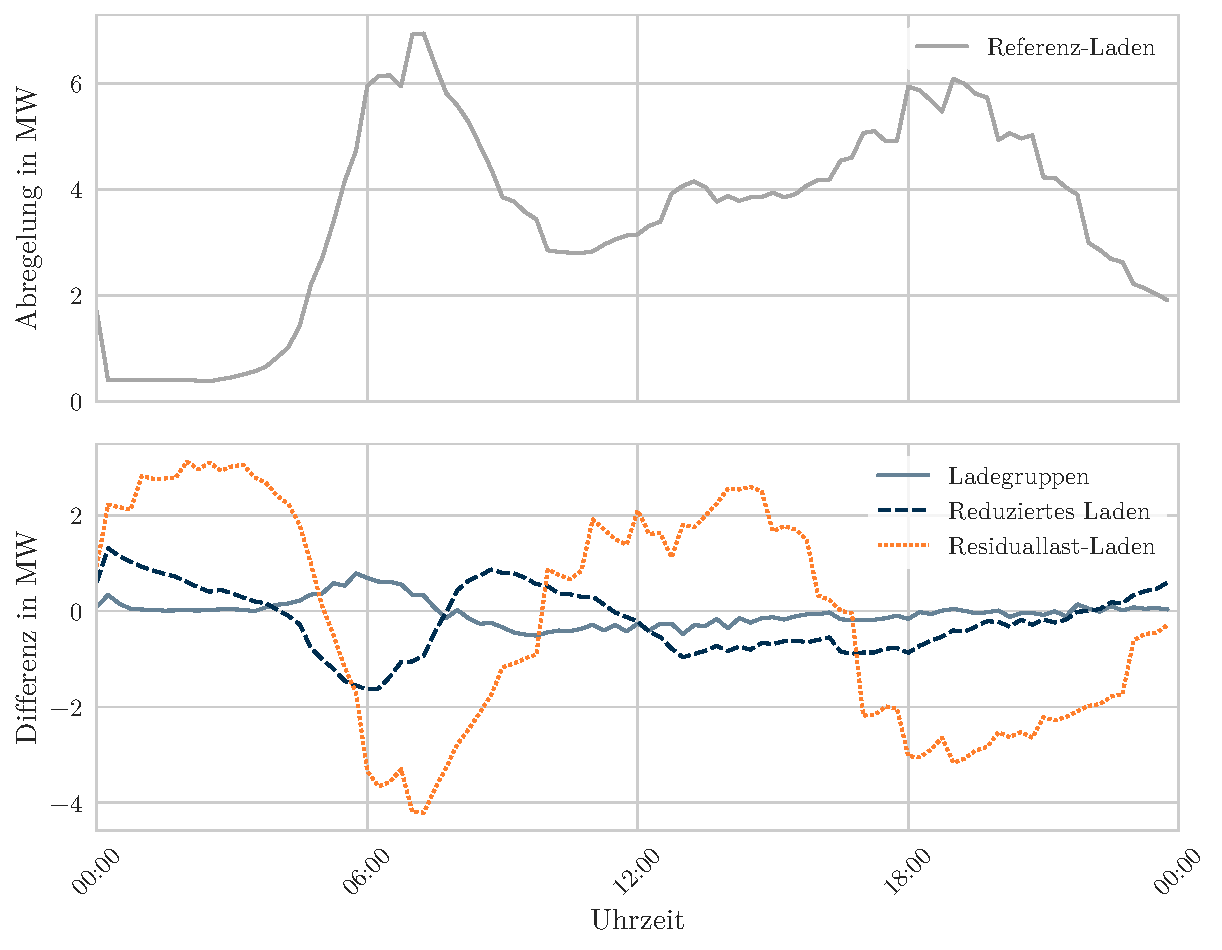
\includegraphics[width=\textwidth]{Bilder/177_load_diff}
    \caption{Durchschnittliche Abregelung von Lasten (oben) innerhalb von Woche~MIN und die durchschnittliche Differenz des Abregelungsbedarfs der Ladestrategien gegenüber dem Referenz-Laden für Lasten (unten) im Antriebswende-Szenario im Netz \num{177}}\label{fig:177_load_diff}
\end{figure}

\autoref{fig:177_load_diff}

{
\renewcommand{\arraystretch}{1.2}% grßerer Zeilenabstand
\sisetup{range-phrase=~{--}~}% Gedankenstrich statt "bis" bei SIrange
\begin{table}[H]
	\begin{center}
		\caption{Abregelungsbedarf von fEE Anlagen im Last-domnierten Netz je Szenario für die Referenz-Ladestrategie}
		\begin{tabu} to 0.6\textwidth {X[1.5] X[1, r] X[1, r]}
			\toprule
			Abregelung in   \si{\mwh}    & Woche A   & Woche B   \\ \midrule
			NEP C~\num{2035}             & \num{0.7} & \num{0.0} \\
			Referenz                     & \num{0.5} & \num{0.0} \\
			Antriebswende                & \num{0.3} & \num{0.0} \\
			\glqq Firmenparkplatz\grqq{} & \num{0.2} & \num{0.0} \\ \bottomrule
		\end{tabu}
		\label{tab:load_dominated_fee_cur}
	\end{center}
	\vspace{-3mm}%Put here to reduce too much white space after your table
\end{table}
}

\autoref{tab:load_dominated_fee_cur}

\begin{figure}[H]
    \centering
    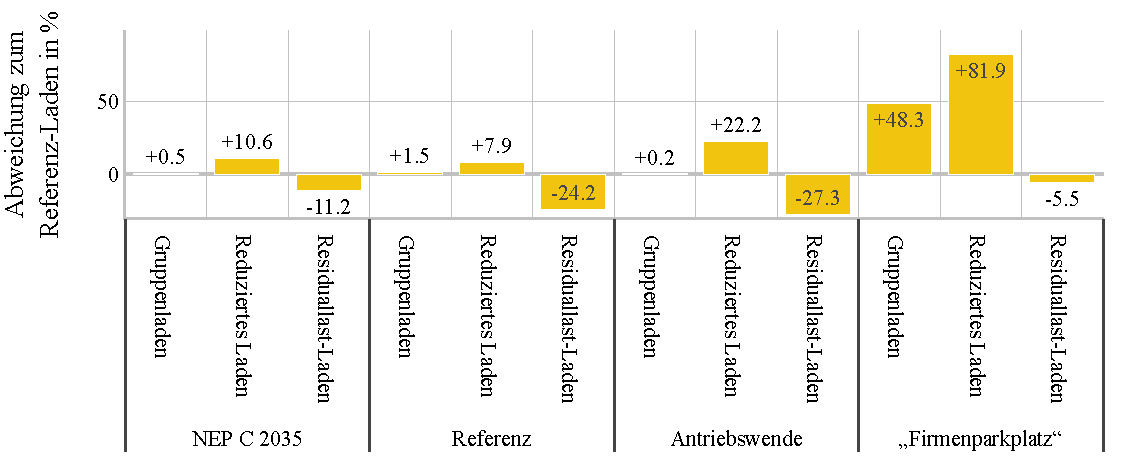
\includegraphics[width=\textwidth]{Bilder/177_cur_fee_grid_week_A}
    \caption[Prozentuale Veränderung des Abregelungsbedarfs von fEE Anlagen in Abhängigkeit von der Ladestrategie in Woche~MIN gegenüber dem Abregelungsbedarf für die Referenz-Ladestrategie je Szenario für das Netze \num{177}]{Prozentuale Veränderung des Abregelungsbedarfs von fEE Anlagen in Abhängigkeit von der Ladestrategie in Woche~MIN gegenüber dem Abregelungsbedarf für die Referenz-Ladestrategie je Szenario für das Netze \(177_{\text{L}}\)}\label{fig:177_cur_fee_grid_week_A}
\end{figure}

\autoref{fig:177_cur_fee_grid_week_A}



\clearpage
